\documentclass[review,12pt]{elsarticle}

% --- Core packages ------------------------------------------
\usepackage{amsmath,amssymb}
\usepackage{bm}
\usepackage{graphicx}
\usepackage{booktabs}
\usepackage{multirow}
\usepackage{array}
\usepackage{tabularx}
\usepackage{longtable}
\usepackage{caption}
\usepackage{subcaption}
\usepackage{xcolor}
\usepackage{url}
\usepackage{hyperref}
\usepackage{microtype}
\usepackage{enumitem}
\usepackage{cleveref}
\sloppy
\graphicspath{{figures/}{./}}

% --- Table column types -------------------------------------
\newcolumntype{L}[1]{>{\raggedright\arraybackslash}p{#1}}
\newcolumntype{C}[1]{>{\centering\arraybackslash}p{#1}}
\newcolumntype{R}[1]{>{\raggedleft\arraybackslash}p{#1}}

% ===========================================================
\begin{document}

\begin{frontmatter}

\title{Whole Field Methods for Fringe Order Demodulation Using Machine Learning Approach in Digital Photoelasticity}

\author[inst1]{[Author Name(s)]\corref{cor1}}
\cortext[cor1]{Corresponding author}
\ead{author@institution.edu}

\affiliation[inst1]{organization={Department of Mechanical Engineering, Institution Name},
             city={City},
             country={Country}}

\begin{abstract}
Digital photoelasticity is a hi well-established full-field optical technique
for experimental stress analysis of engineering components. The reliable
determination of the isochromatic fringe order $N$ across the entire field
of view---whole-field fringe order demodulation---remains a central
challenge, particularly under variable illumination and for complex specimen
geometries. Classical approaches including RGB three-fringe photoelasticity
\cite{ajovalasit1995,ramesh1996}, multi-step phase-shifting
\cite{wang1995,siegmann2005}, and Fourier-transform-based methods
\cite{quan1993} each impose constraints on experimental setup, fringe
density, or number of image acquisitions. Recent deep learning approaches
have demonstrated promising results \cite{tao2022,naranjo2022,mohan2024}
but are parameter-intensive and require large labelled training sets.

This paper proposes a whole-field, single-image fringe order demodulation
framework based on extreme gradient-boosted decision trees (XGBoost)
\cite{chen2016}. At inference the method requires only a single RGB
isochromatic image and predicts the fractional fringe order $\hat{N}$ at
every pixel; no knowledge of applied load, specimen geometry, or material
constants is used. A dual-model architecture predicts the sine and cosine
of $2\pi N$ independently, eliminating the circular discontinuity at integer
fringe orders, with the fractional fringe order recovered via
$\mathrm{arctan2}$. Models are trained on a large combined dataset of
physics-simulated synthetic fringe images rendered for three specimen
geometries across ten spectral conditions, together with geometrically
augmented real experimental images. Each pixel is described by a
27-dimensional feature vector encoding colour, neighbourhood statistics,
gradient, Laplacian, and multi-scale Gabor filter responses. GPU-accelerated
training ingests a ${>}70$~GB dataset in memory-efficient chunks.
Experimental validation on unseen ring and disc specimens demonstrates
RMSE~$= 0.1112$ fringe orders on the synthetic test set ($R^2 = 0.8485$).
The method is calibration-free, illumination-robust, and deployable across
arbitrary specimen geometries without retraining.
\end{abstract}

\begin{keyword}
digital photoelasticity \sep fringe order demodulation \sep XGBoost \sep
machine learning \sep isochromatic fringes \sep whole-field measurement \sep
synthetic dataset \sep RGB photoelasticity \sep stress analysis
\end{keyword}

\end{frontmatter}

% ===========================================================
\section{Introduction}
\label{sec:intro}
Photoelasticity is a key method for stress analysis. It has been used since the early 1900s.
Polarized white light passes through a birefringent specimen under load.
This creates isochromatic fringe patterns on a color camera.
These patterns display the main stress difference $(\sigma_1 - \sigma_2)$ at each visible point, based on the stress-optic law \cite{dally1991}.
Photoelasticity is full-field, non-contact, and non-destructive.
These features attract its use in aerospace, biomedical, civil, and manufacturing engineering \cite{ramesh2015,patterson2002}.

The main task in quantitative digital photoelasticity is to find the isochromatic fringe order N for each pixel. According to the stress-optic law, $N = hC(\sigma_1 - \sigma_2)/\lambda$, where $h$ is the specimen thickness, $C$ the stress-optic coefficient, and $\lambda$ the wavelength of light \cite{dally1991}. Accurate whole-field $N$ extraction means recovering the full principal stress difference field. This is the main goal of quantitative photoelastic analysis.

Automated demodulation has followed three principal strategies over the past three decades. RGB three-fringe photoelasticity (TFP) was first introduced by Ajovalasit et al.\ \cite{ajovalasit1995} and further developed by Ramesh and his team \cite{ramesh1996,ramesh2011,madhu2007}. It finds $N$ by comparing the measured RGB triple to a calibration look-up table specific to the material. TFP is simple because it needs just one image. However, it is sensitive to changes in lighting. When N is 3 or more, it can be unclear without extra scanning refinement \cite{kale2013,ramesh2015}. Phase-shifting methods \cite{wang1995,ramesh1996phaseshifting,siegmann2005} capture several images at set optical retarder steps. This offers precise whole-field demodulation. However, it requires extra hardware and multiple captures, which limits dynamic measurements. Fourier-transform and carrier-frequency methods \cite{quan1993,morimoto1994} let you demodulate a single image. This happens in the spatial frequency domain. However, they need a minimum carrier fringe density, which limits where they can be used. A comprehensive review of classical approaches is given in \cite{ajovalasit2015,ramesh2021}.

The rapid maturation of machine learning (ML) has motivated its application across optical metrology \cite{zhu2022}. Deep convolutional neural networks (CNNs) are used in digital photoelasticity for several tasks. They help with isochromatic fringe pattern segmentation \cite{brinezdeleon2022}. They also recover stress fields from single images \cite{tao2022,naranjo2022} and demodulate whole-field fringe orders \cite{mohan2024}. FringeNet \cite{mohan2024} stands out. It is a cyclic U-Net design. It uses a special loss called Continuity-Imposed Hybrid Cyclic Loss (CHCL). This design leads to a 92.4\% improvement in MSE and a 16.19\% boost in PSNR compared to other methods on the IsochromaticArt benchmark. Bri\~nez-de Le\'{o}n et al.\ \cite{brinezdeleon2024} offer a detailed review of deep learning in digital photoelasticity. They highlight three main challenges: dataset scarcity, interpretability, and generalization.

Gradient-boosted decision trees, especially XGBoost, provide a top-notch method for structured tabular regression. This approach is easy to interpret using gain-based feature importance. It is also efficient on GPU hardware, thanks to histogram-based split-finding. XGBoost is used to predict mechanical properties \cite{shi2023} and estimate structural stress \cite{vivekanandan2020}. No one has reported using it for pixel-level photoelastic fringe order demodulation over entire fields. This paper addresses this gap.

The specific contributions of this work are:

\begin{enumerate}[label=(\alph*)]

\item A physics-based pipeline for synthetic fringe image generation
spanning three specimen geometries: beam under pure bending, plate with a
circular hole under uniaxial tension (Kirsch solution), and diametrically
loaded disc (Timoshenko solution). The images are rendered under ten
spectral conditions obtained from five illuminant spectral power
distributions (SPDs) and two RGB sensor sensitivity profiles. Multiple
load levels are used solely to generate a diverse range of fringe
densities and colour distributions; load values are not used as model
inputs.

\item A geometric augmentation strategy for BMP--FRN pairs that applies
identical spatial transformations to both the image and the corresponding
ground-truth fringe-order map, thereby preserving exact pixel-to-fringe-order
correspondence. This procedure generates 25 augmented pairs from each
original sample.

\item A 27-dimensional pixel-level feature descriptor derived exclusively
from the RGB image, comprising normalised RGB colour, circular hue
encoding, saturation, local neighbourhood statistics, bilateral filter
responses, local range, gradient magnitudes, Laplacian responses, and
multi-scale Gabor filter outputs at four orientations.

\item A dual XGBoost regression framework employing
$\sin(2\pi N)$ and $\cos(2\pi N)$ as separate targets, with the fractional
fringe order recovered using the $\mathrm{arctan2}$ function. This
formulation eliminates the circular discontinuity at integer fringe
orders, which otherwise degrades direct scalar regression.

\item Experimental validation on ring and disc specimens not included in
the training data or synthetic geometry set. The model is evaluated using
RMSE, $R^2$, and MAE against ground-truth fringe-order maps obtained via a
standard phase-stepping procedure. All evaluation metrics are reported
exclusively in the fringe-order domain.

\end{enumerate}

The remainder of the paper is organised as follows. Section~\ref{sec:related}
reviews related work. Section~\ref{sec:methodology} presents the complete
methodology. Section~\ref{sec:experiment} describes the experimental programme.
Section~\ref{sec:results} presents quantitative results. Section~\ref{sec:discussion}
discusses findings, limitations, and comparisons. Section~\ref{sec:conclusion}
concludes.

% ===========================================================
\section{Related Work}
\label{sec:related}

\subsection{Classical Fringe Order Demodulation}

Automated fringe order demodulation in photoelasticity has a history spanning over three decades. Ajovalasit, Barone, and Petrucci \cite{ajovalasit1995} started RGB photoelasticity. They matched one white-light isochromatic image to a color calibration look-up table (LUT). This helped them determine the retardation. Ramesh and Deshmukh \cite{ramesh1996} made three-fringe photoelasticity (TFP). Later, their team added new strategies. These are advancing-front \cite{kale2013} and fringe-resolution-guided \cite{ramesh2015}. They help improve reliable demodulation for higher fringe orders. Ajovalasit, Petrucci, and Scafidi \cite{ajovalasit2015} provide a comprehensive review of RGB photoelasticity. Ramesh et al.\ \cite{ramesh2011} and Madhu and Ramesh \cite{madhu2007} looked into issues with nonuniqueness and color adaptation under various light sources. The software packages PSCOPE\textsuperscript{\textregistered} and DigiTFP\textsuperscript{\textregistered} from IIT Madras combine proven TFP algorithms into one platform \cite{ramesh2015pscope,ramesh2015digitfp}.

Phase-shifting methods offer better accuracy, but they require more acquisitions and extra hardware. Wang and Patterson \cite{wang1995} combined phase-stepping with fuzzy-set processing. Ramesh and Ganapathy \cite{ramesh1996phaseshifting} formalized the methodology using Jones calculus. Siegmann, Backman, and Patterson \cite{siegmann2005} showed a strong method. It focuses on regions to handle complex fringe patterns. This is useful for aerospace samples. Ramji and Ramesh \cite{ramji2010} created an adaptive algorithm. It guides quality in unwrapping isoclinic and isochromatic phasemaps. Phase ambiguity and unwrapping for isochromatic maps are treated in \cite{ramesh2004,ramji2008}.

Fourier-transform and carrier-frequency methods \cite{quan1993,morimoto1994} allow single-image demodulation. They work in the spatial frequency domain. Regularization and color-difference methods \cite{quiroga1997,swain2014} increase TFP to higher fringe orders. However, all classical methods have drawbacks. They are sensitive to illuminants, require material calibration, or are complex to set up.

\subsection{Machine Learning and Deep Learning in Photoelasticity}

The application of ML to digital photoelasticity has accelerated substantially since 2018. Zhu et al.\ \cite{zhu2022} offer a wide review of deep learning in optical metrology. They discuss interferometry, holography, and photoelasticity. In digital photoelasticity, Tao et al.\ \cite{tao2022} introduced a CNN encoder-decoder. It recovers the principal stress difference map from one isochromatic image. This shows that end-to-end deep learning is feasible. Naranjo and Restrepo-Mart\'{i}nez \cite{naranjo2022} used deep CNNs. They extracted stress fields from multi-polarised photoelasticity images. Bri\~nez-de Le\'{o}n et al.\ \cite{brinezdeleon2024} offer a critical review from 2018 to 2024. They mention three main challenges. First, there is dataset scarcity. Second, interpretability is an issue. Third, generalization in different lighting conditions is a challenge.

The closest previous work is FringeNet \cite{mohan2024}. It features a cyclic U-Net design. It was trained on the open-source Isochromatic-Art dataset. FringeNet uses a Continuity-Imposed Hybrid Cyclic Loss (CHCL). This combines MSE, SSIM, PSNR, and a spatial continuity penalty. Together, these elements help ensure fringe order smoothness. It shows a 92.4\% boost in MSE and a 16.19\% increase in PSNR compared to other methods on the Isochromatic-Art benchmark. Validation on experimental disc and ring images achieves an average SSIM of 0.85. FringeNet's sin/cos output is similar to the dual-target encoding here. The main difference is that FringeNet uses a U-Net backbone that is aware of spatial context. This work uses hand-crafted neighborhood and texture features. It relies on a gradient-boosted ensemble. This approach allows for clear physical interpretability through gain-based feature importance.

Beyond photoelasticity, gradient-boosted methods have achieved state-of-the-art performance on structured engineering regression tasks. Shi et al.\ \cite{shi2023} showed that XGBoost can predict stress in lattice structures with defects. They achieved an $R^2$ value greater than 0.95. Gradient-boosted trees are generally better than deep networks for tabular data. This is well known \cite{chen2016,prokhorenkova2018}. The authors think this is the first use of XGBoost with trigonometric target encoding. It applies to whole-field photoelastic fringe order demodulation.

\subsection{Synthetic Data and Augmentation in Photoelasticity}

Dataset scarcity is the principal bottleneck for supervised learning in photoelasticity \cite{brinezdeleon2024}. Physics-based simulation provides a principled route to large annotated datasets. The Isochromatic-Art dataset \cite{mohan2024} has over 100,000 synthetic isochromatic image pairs. This is great for researchers. This work builds on earlier studies by altering the specimen shape and lighting setup. We look at three analytical solutions. For each shape-load pair, there are ten conditions. We use five illuminants and two sensor profiles. This creates a training distribution with a wider variety of lighting. Data augmentation using geometric transforms is common in computer vision \cite{shorten2019}. However, in photoelasticity, there is an important extra rule. The BMP image and its ground-truth FRN map must get the same spatial transform. This keeps the pixel-to-fringe-order correspondence intact. Such a rule is not needed in standard image classification tasks.

% ===========================================================
\section{Methodology}
\label{sec:methodology}

The complete pipeline, shown in Fig.~\ref{fig:pipeline}, comprises four stages:
(i) synthetic fringe image generation, (ii) real image augmentation,
(iii) pixel level feature extraction, and (iv) dual XGBoost model training.
It is essential to understand the role of physical quantities in this
pipeline: applied loads and stress solutions appear \emph{only} in Stage~(i)
to produce image ground truth pairs. From Stage~(ii) onward, the pipeline
operates exclusively on pixel-level RGB data and its derived features. The
trained model therefore has no dependence on load, specimen geometry, or
material constants at inference time.

\begin{figure}[htbp]
  \centering
  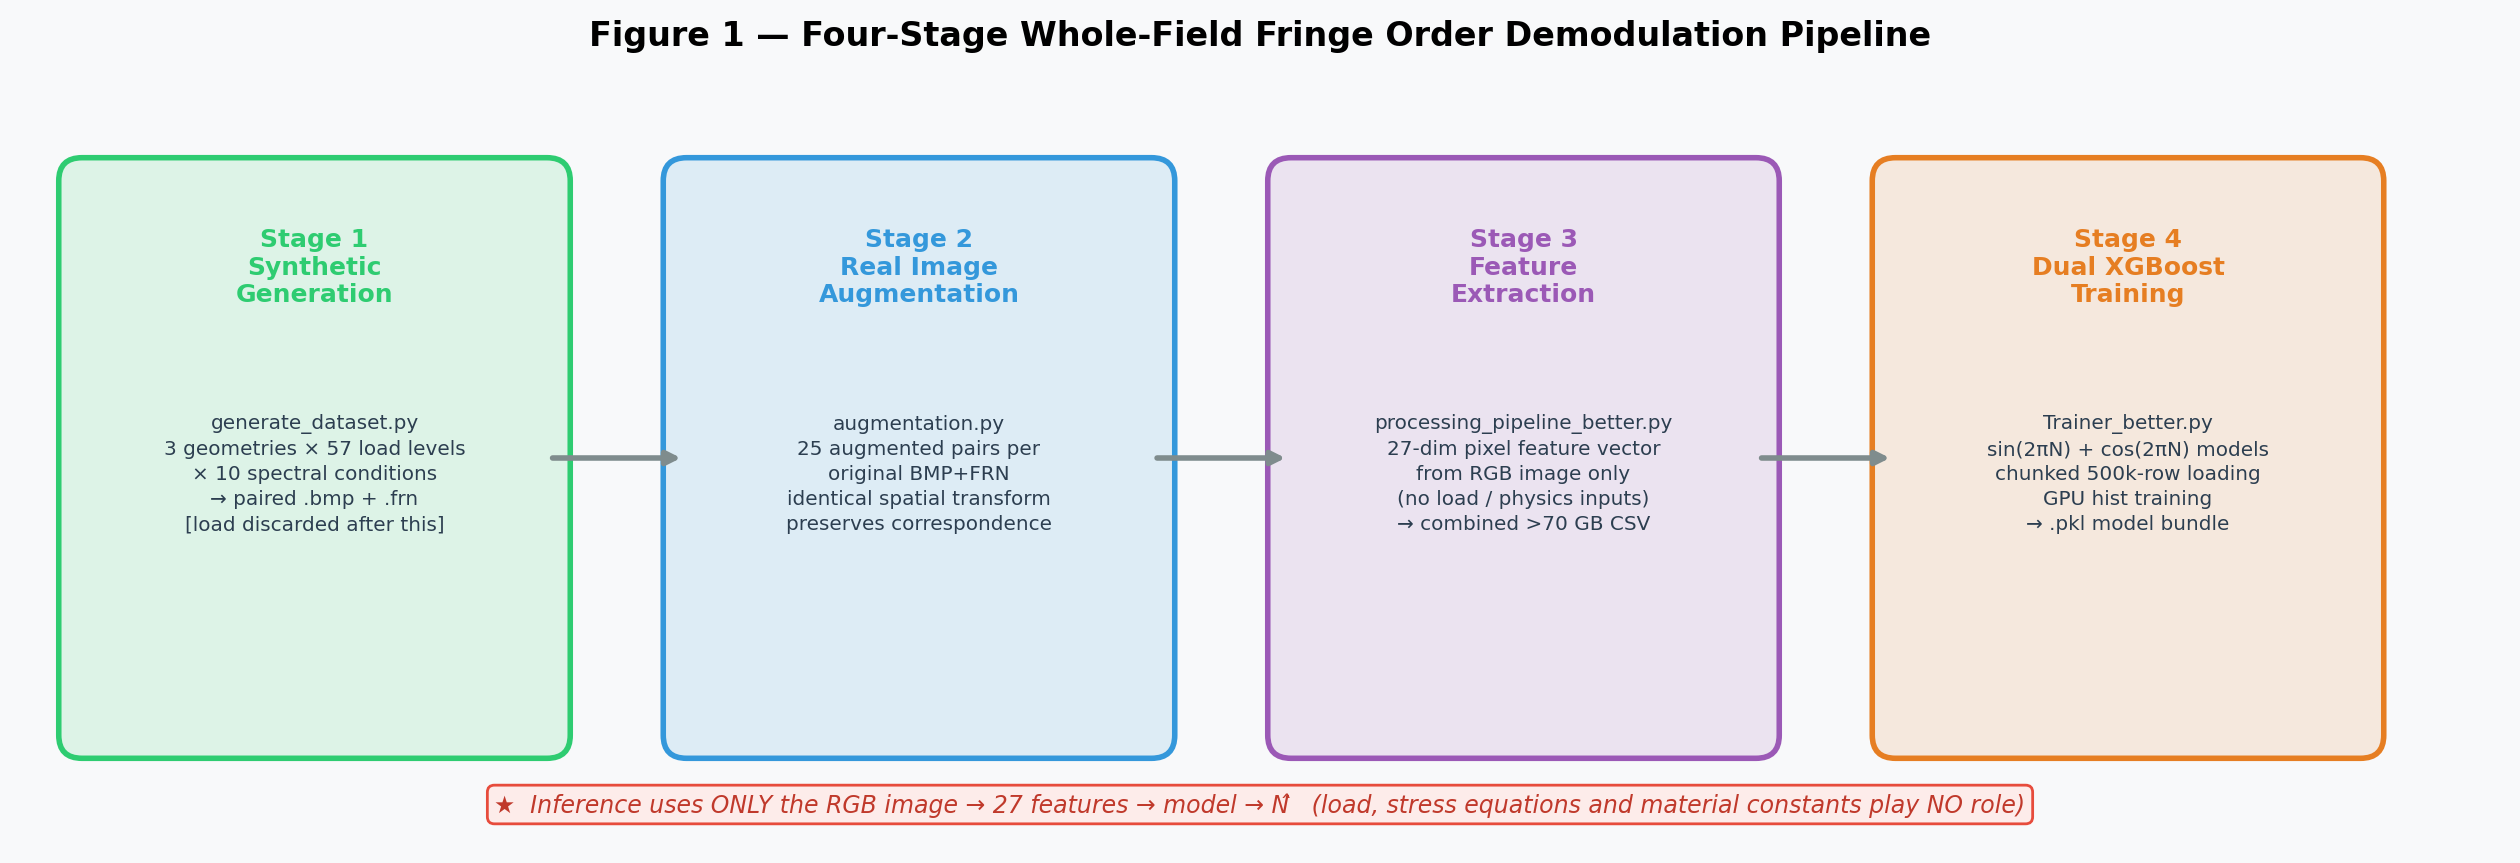
\includegraphics[width=0.96\linewidth]{Fig1_pipeline}
  \caption{Overview of the proposed whole-field fringe order demodulation
    pipeline. Synthetic and augmented real image pairs are processed into a
    unified pixel level dataset, which trains dual XGBoost regressors.
    The fractional fringe order $\hat{N}$ is recovered at every pixel via
    $\mathrm{arctan2}$ from the RGB image alone.}
  \label{fig:pipeline}
\end{figure}

\subsection{Theoretical Background}
\label{sec:theory}

In a dark-field circular polariscope, the isochromatic fringe pattern is
formed free from isoclinic contamination \cite{dally1991,ramesh2000}. For
a birefringent specimen of thickness $h$ and stress-optic coefficient $C$,
the optical retardation introduced at wavelength $\lambda$ by principal
stresses $\sigma_1$ and $\sigma_2$ is:
\begin{equation}
  \delta(\lambda) = \frac{2\pi h C (\sigma_1 - \sigma_2)}{\lambda}
  \label{eq:retardation}
\end{equation}

Under the dark-field configuration, the transmitted intensity at wavelength
$\lambda$ is:
\begin{equation}
  I(\lambda) = I_0(\lambda)\,\sin^2\!\left[\delta(\lambda)/2\right]
  \label{eq:intensity}
\end{equation}

The isochromatic fringe order is defined as:
\begin{equation}
  N = \frac{\delta}{2\pi} = \frac{h C (\sigma_1 - \sigma_2)}{\lambda}
  \label{eq:fringeorder}
\end{equation}

For a colour camera with per-channel spectral sensitivity $r_c(\lambda)$,
$c \in \{R,G,B\}$, illuminated by source SPD $S(\lambda)$, the digital
response in channel $c$ is:
\begin{equation}
  R_c = \int_{390}^{760} I(\lambda)\,S(\lambda)\,r_c(\lambda)\,\mathrm{d}\lambda
  \label{eq:camera}
\end{equation}

Equation~\eqref{eq:camera} establishes the physical basis for using the RGB
image alone to infer fringe order. The resulting $(R,G,B)$ triplet is
non-unique for $N \gtrsim 3$ under most broadband illuminants
\cite{ajovalasit2015}, motivating training across multiple spectral
conditions (Section~\ref{sec:spectral}). Only the fractional part
$N \bmod 1 \in [0,1)$ is predicted; integer $N$ recovery requires a
subsequent unwrapping step not addressed here.

\textbf{Note.} Equations~\eqref{eq:retardation}--\eqref{eq:camera}
are used exclusively in the synthetic data generation pipeline
(Section~\ref{sec:synthetic}) to compute ground-truth $N$ maps and render
the corresponding RGB images. The trained model receives only the pixel's
27-dimensional image feature vector (Section~\ref{sec:features}) and
outputs $\hat{N}$ directly.

\subsection{Synthetic Dataset Generation}
\label{sec:synthetic}


A large physics-based synthetic dataset was created. It used closed-form analytical stress solutions for three specimen shapes. This was done in\texttt{generate\_dataset.py}. Applied loads in this stage control the fringe density of the image. A higher load means denser fringes and a broader range of N values. Their main job is to fill the training distribution with images. These images should cover a wide variety of fringe densities and color combinations. This approach follows the synthetic-data strategy established i n\cite{mohan2024,brinezdeleon2024}. For each geometry-spectral combo, we create two files. One is an 8-bit RGB BMP image. It measures ($602 \times 461$ pixels,
0.5~mm/pixel). The other file is a tab-separated fringe-order ground-truth map (\texttt{.frn}).
\subsubsection{Specimen geometries}

\paragraph{Beam under pure bending.}
Euler--Bernoulli bending stress in a rectangular cross-section ($b = 6$~mm,
$h_b = 10$~mm):
\begin{equation}
  \sigma(y) = \frac{My}{I}, \qquad I = \frac{b\,h_b^3}{12}
  \label{eq:beam}
\end{equation}
Thirty-seven bending moment values spanning $M \in [100, 975]$~N$\cdot$m
were used during dataset generation to produce images with varying fringe
densities.

\paragraph{Plate with circular hole under uniaxial tension.}
Kirsch solution \cite{kirsch1898} for an infinite plate with hole radius
$a = 25$~mm under far-field stress $\sigma_\infty$:
\begin{align}
  \sigma_r    &= \frac{\sigma_\infty}{2}\!\left(1-\frac{a^2}{r^2}\right)
                 + \frac{\sigma_\infty}{2}\!\left(1-\frac{4a^2}{r^2}
                 + \frac{3a^4}{r^4}\right)\!\cos 2\theta \label{eq:kirsch_r}\\
  \sigma_\theta &= \frac{\sigma_\infty}{2}\!\left(1+\frac{a^2}{r^2}\right)
                 - \frac{\sigma_\infty}{2}\!\left(1+\frac{3a^4}{r^4}\right)
                 \!\cos 2\theta \label{eq:kirsch_theta}\\
  \tau_{r\theta} &= -\frac{\sigma_\infty}{2}\!\left(1+\frac{2a^2}{r^2}
                 - \frac{3a^4}{r^4}\right)\!\sin 2\theta \label{eq:kirsch_tau}
\end{align}
Six far-field stress values $\sigma_\infty \in \{0.5, 1.0, 1.5, 2.0, 2.5,
3.0\}$~MPa were used as data-generation parameters.

\paragraph{Diametrally loaded disc.}
Timoshenko and Goodier \cite{timoshenko1970} solution for a disc of radius
$R = 30$~mm and thickness $t = 6$~mm under load $P$:
\begin{align}
  \sigma_x &= -\frac{2P}{\pi t}\!\left[\frac{s\,x^2}{a^2}
               + \frac{q\,x^2}{b^2} - \frac{1}{2R}\right] \label{eq:disc_sx}\\
  \sigma_y &= -\frac{2P}{\pi t}\!\left[\frac{s^3}{a^2}
               + \frac{q^3}{b^2} - \frac{1}{2R}\right] \label{eq:disc_sy}\\
  \tau_{xy} &= -\frac{2P}{\pi t}\!\left[\frac{q^2 x}{b^2}
               - \frac{s^2 x}{a^2}\right] \label{eq:disc_txy}
\end{align}
where $s = R-y$, $q = R+y$, $a^2 = x^2+s^2$, $b^2 = x^2+q^2$. Fourteen
load values $P \in \{10.1, 12.0, 13.9, 15.9, 17.8, 19.7, 21.7, 23.6,
25.5, 27.5, 29.4, 31.3, 33.3, 35.2\}$~N were used as data-generation
parameters.

\subsubsection{Spectral conditions}
\label{sec:spectral}

Each geometry is shown under  $N_\mathrm{spec} = 10$ spectral conditions. This includes five illuminant SPDs and two RGB sensor sensitivities (Table~\ref{tab:spectral}). The spectral axis spans $\lambda \in [390, 760]$~nm  at 371 uniformly spaced wavelength steps. The spectral integration ofEq. ~\eqref{eq:camera} is calculated numerically. We use the trapezoidal rule with CuPy/CUDA for GPU array operations. If needed, we fall back to NumPy. The resulting RGB image is per-channel min-max normalised to $[0,255]$ and saved as an 8-bit BMP. The ground-truth fringe-order map is stored as a single-precision float32 .frn file. Rendering under ten spectral conditions mixes up the training data from any one illuminant-sensor pair. This makes the model strong against changes in lighting\cite{ajovalasit2015,madhu2007b}.

\begin{table}[htbp]
  \centering
  \caption{Spectral conditions used for synthetic image generation
    (5 illuminants $\times$ 2 sensors $= 10$ conditions per geometry).}
  \label{tab:spectral}
  \footnotesize
  \begin{tabular}{@{}p{1.2cm}p{4.2cm}p{3.5cm}p{4.5cm}@{}}
    \toprule
    ID    & Illuminant SPD $S(\lambda)$          & Sensor $r_c(\lambda)$
          & Source \\
    \midrule
    S1--C1 & White broadband (measured)           & Sony IMX (measured)
           & Calibrated spectral database \\
    S1--C2 & White broadband (measured)           & Gaussian RGB analytic
           & Peaks 650/547/460~nm, $\sigma=20$~nm \\
    S2--C1 & Fluorescent (measured)               & Sony IMX (measured)
           & Calibrated spectral database \\
    S2--C2 & Fluorescent (measured)               & Gaussian RGB analytic
           & Peaks 650/547/460~nm, $\sigma=20$~nm \\
    S3--C1 & Incandescent (measured)              & Sony IMX (measured)
           & Calibrated spectral database \\
    S3--C2 & Incandescent (measured)              & Gaussian RGB analytic
           & Peaks 650/547/460~nm, $\sigma=20$~nm \\
    S4--C1 & Multi-peak Gaussian fluorescent      & Sony IMX (measured)
           & Peaks at 435,545,580,610~nm; amps 0.1,0.2,0.3,0.4 \\
    S4--C2 & Multi-peak Gaussian fluorescent      & Gaussian RGB analytic
           & As S4-C1 \\
    S5--C1 & Broadband green LED Gaussian         & Sony IMX (measured)
           & Peak 550~nm, $\sigma=50$~nm \\
    S5--C2 & Broadband green LED Gaussian         & Gaussian RGB analytic
           & Peak 550~nm, $\sigma=50$~nm \\
    \bottomrule
  \end{tabular}
\end{table}

\begin{table}[htbp]
  \centering
  \caption{Synthetic dataset dimensions by geometry.}
  \label{tab:dataset_dims}
  \small
  \begin{tabular}{@{}lcccc@{}}
    \toprule
    Geometry & Load levels (data gen.\ only) & Spectral cond. & Image pairs & $N_\mathrm{max}$ (approx.) \\
    \midrule
    Beam (bending)        & 37 (100--975 N$\cdot$m, $\Delta=25$ N$\cdot$m) & 10
      & 370 & $\sim$12 \\
    Plate-with-hole       & 6 (0.5--3.0 MPa, $\Delta=0.5$ MPa)             & 10
      & 60 & $\sim$5 \\
    Disc (diametral)      & 14 (10.1--35.2 N, equal spacing)                & 10
      & 140 & $\sim$8 \\
    \midrule
    Total                 & 57 load levels & 10 & 570 & --- \\
    \bottomrule
  \end{tabular}
\end{table}

\begin{figure}[htbp]
  \centering
  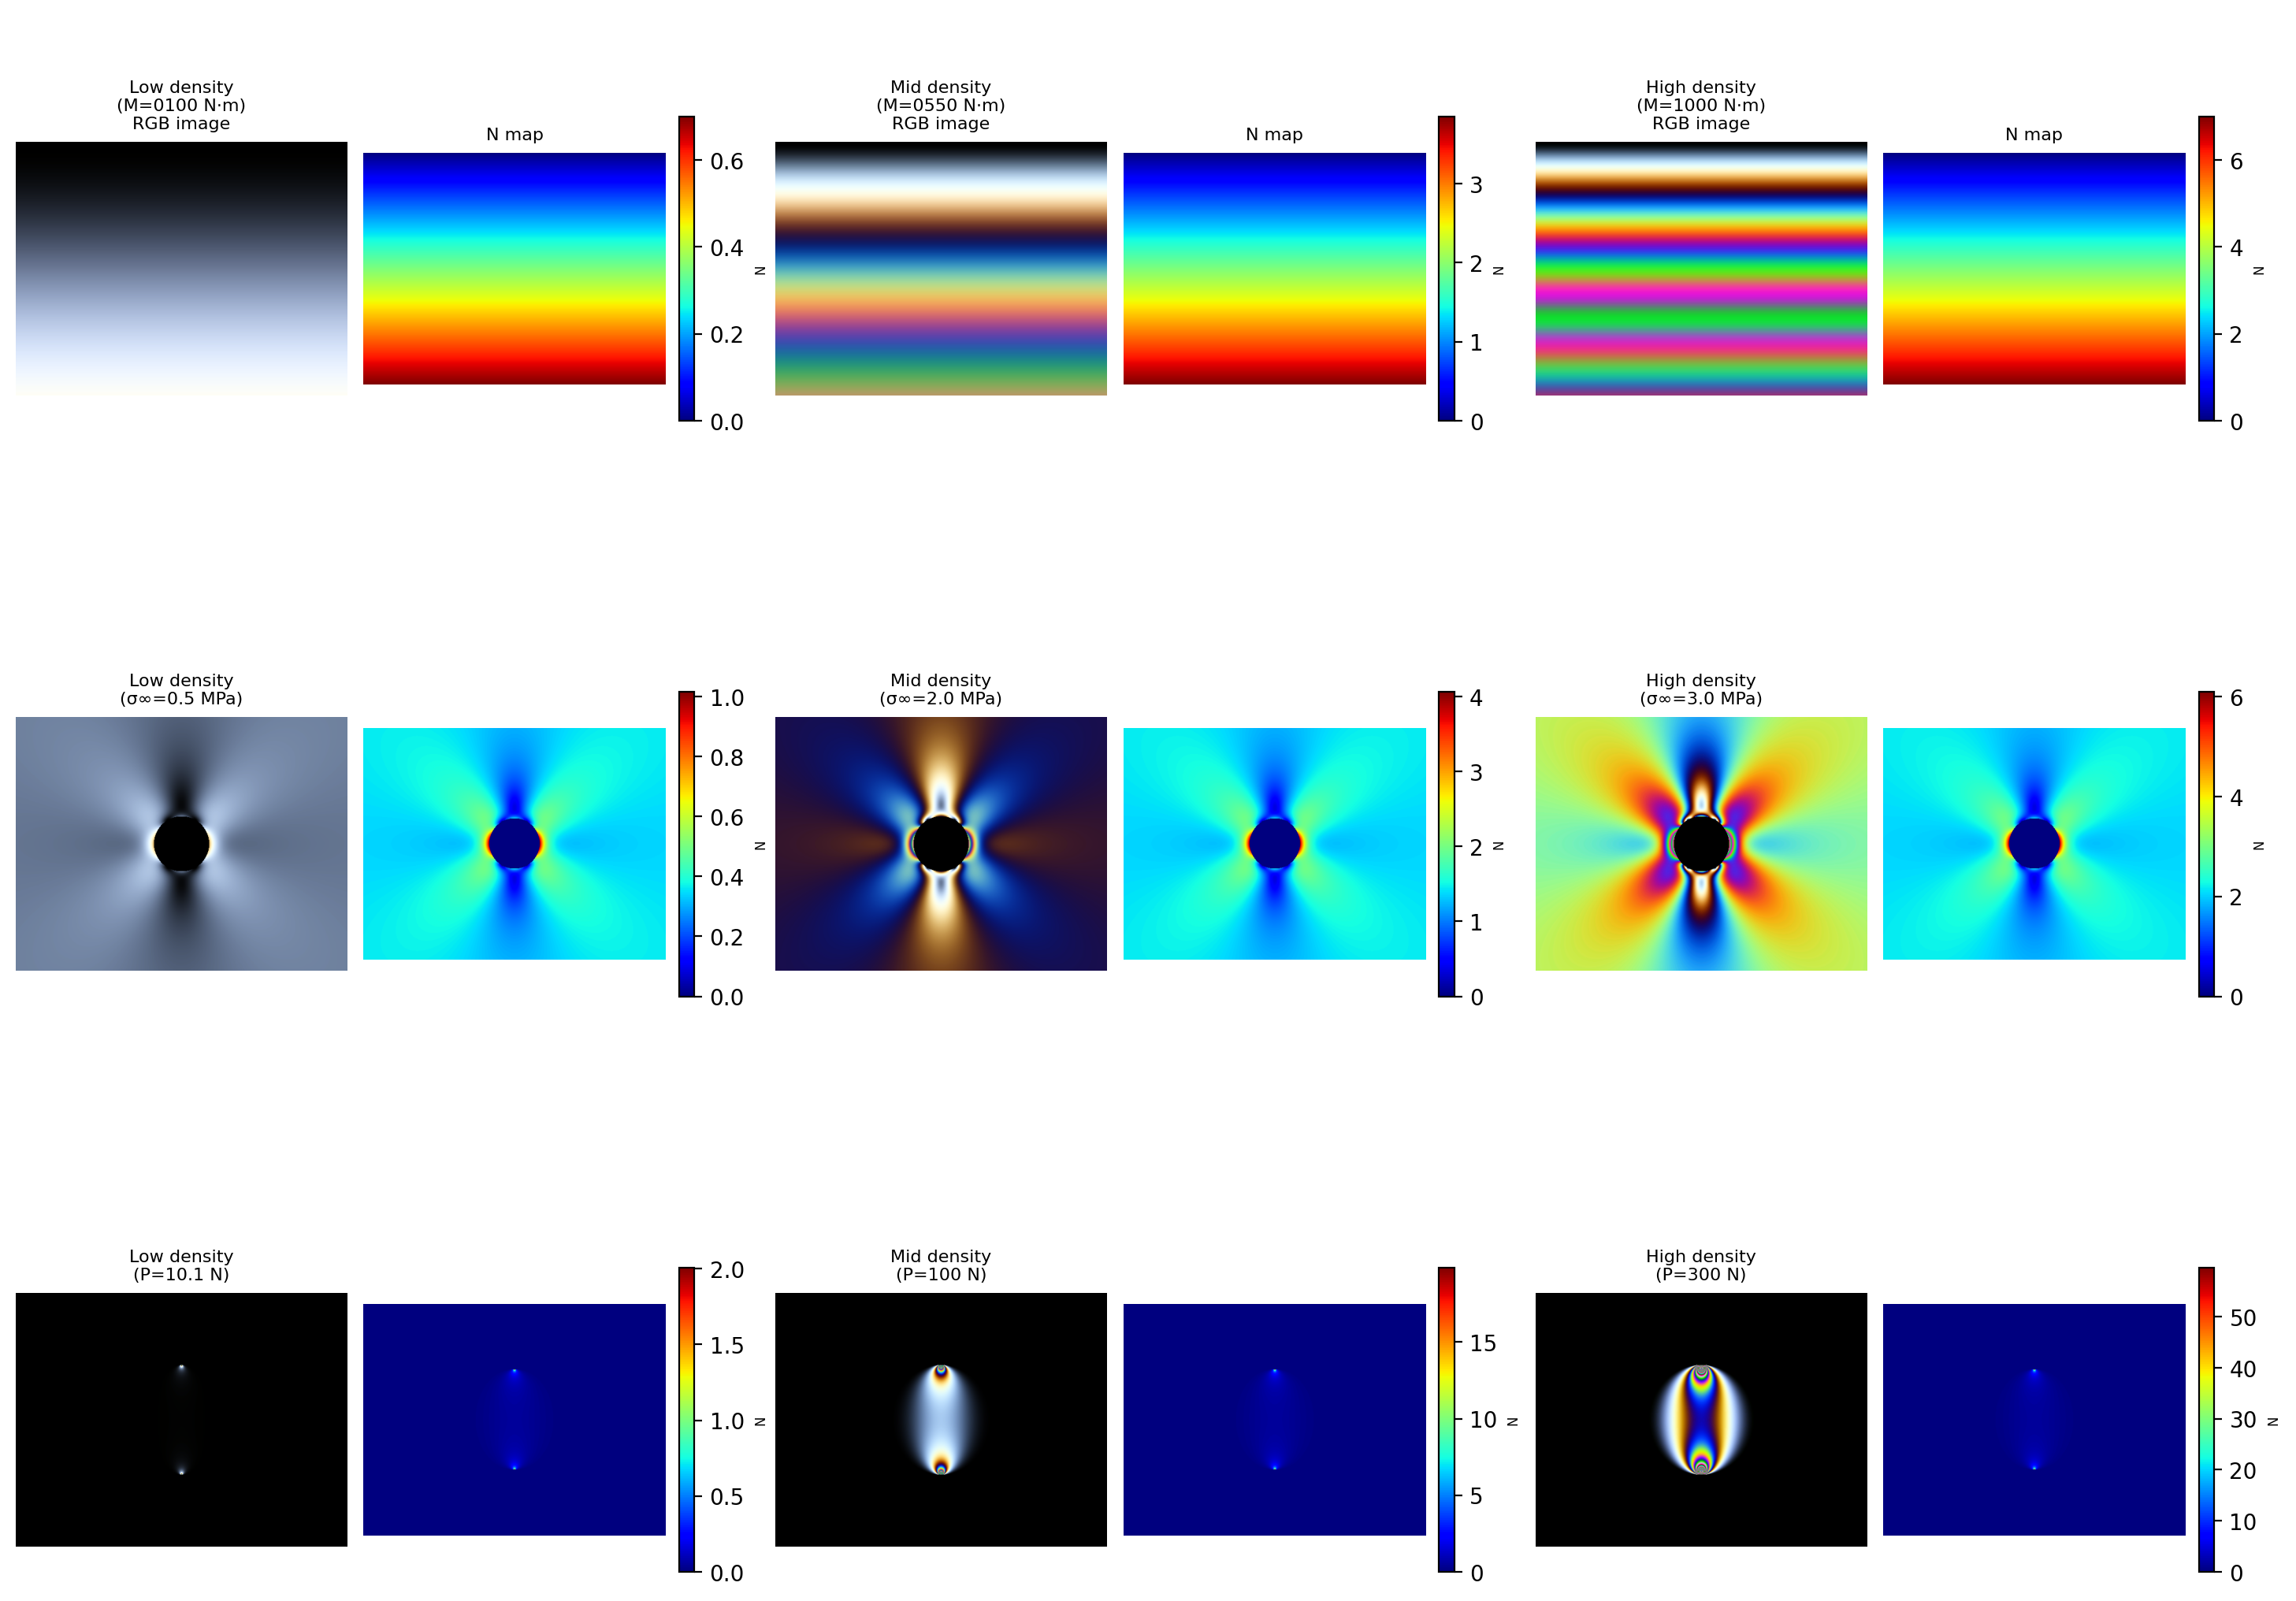
\includegraphics[width=0.96\linewidth]{Fig2_synthetic_grid}
  \caption{Representative synthetic isochromatic fringe images and their
    ground-truth fringe-order maps. Rows: beam
    ($M = 200, 500, 900$~N$\cdot$m), plate-with-hole
    ($\sigma_\infty = 1.0, 2.0, 3.0$~MPa), disc ($P = 12, 21.7, 33.3$~N).
    Load values shown are data-generation parameters that control fringe
    density; they are not model inputs.
    Left sub-panel: normalised RGB image. Right sub-panel: $N$ map.}
  \label{fig:synthetic_grid}
\end{figure}

\subsection{Real Image Augmentation}
\label{sec:augmentation}

Real fringe images were captured using a white-light transmission circular polariscope (Section~\ref{sec:experiment}). Each image is paired with a ground-truth .frn map obtained by phase-stepping. The augmentation pipeline (augmentation.py) creates 25 new BMP–FRN pairs for each original. 

It does this by randomly using three spatial transforms: isotropic scaling, biaxial shearing, and random cropping  (Table~\ref{tab:augmentation}).

The main point is that the same AffineTransform object (skimage.transform) uses bilinear interpolation. This applies to both the BMP and the linked FRN. This keeps the pixel-to-fringe-order match exact. No color transforms are used. Color is the main carrier of fringe-order information  \cite{ajovalasit2015,shorten2019}.
\begin{table}[htbp]
  \centering
  \caption{Augmentation parameter ranges. Identical transform applied to BMP and \texttt{.frn}.}
  \label{tab:augmentation}
  \small
  \begin{tabular}{@{}llll@{}}
    \toprule
    Transform   & Parameter       & Range              & Notes \\
    \midrule
    Scale       & Scale factor $s$ & $[0.80,\ 1.50]$   & Isotropic; bilinear interpolation \\
    Shear ($x$) & Angle $\alpha_x$ & $[-15^\circ,\ +15^\circ]$   & $\tan(\alpha_x) =$ shear coefficient \\
    Shear ($y$) & Angle $\alpha_y$ & $[-15^\circ,\ +15^\circ]$   & Independent of $\alpha_x$ \\
    Crop        & Ratio $c$        & $0.80\times$ scaled size & Fixed; random origin (uniform valid range) \\
    \bottomrule
  \end{tabular}
\end{table}

\subsection{Feature Extraction}
\label{sec:features}

A 27-dimensional feature vector is calculated for each pixel using local RGB data (Table~\ref{tab:features}). All 27 features come only from the RGB image. No load, geometry, or material parameters are part of the feature vector. 

The descriptor includes three types of information:

(i) Absolute color shows fractional fringe order with ~\eqref{eq:camera}. 

(ii) Neighborhood statistics give local context and cut down noise. 

(iii) Texture and edge responses come from gradient, Laplacian, and Gabor filters. They show fringe orientation, density, and how sharp boundaries are.

 

Gabor filters \cite{daugman1985} help localize both spatial frequency and orientation well. They are proven to be effective for recognizing photoelastic fringe patterns \cite{fandino2018}. Four orientations $(0^\circ, 45^\circ, 90^\circ, 135^\circ)$ cover all angles. Two spatial scales (f1, f2) handle different fringe densities in the training set. The bilateral filter \cite{tomasi1998}  is applied with$\sigma_s = 5$~px and $\sigma_r = 25$
intensity units.


\begin{table}[htbp]
  \centering
  \caption{The 27-dimensional pixel-level feature descriptor.}
  \label{tab:features}
  \footnotesize
  \begin{tabular}{@{}L{2.8cm}L{3.5cm}C{0.7cm}L{5.8cm}@{}}
    \toprule
    Group & Feature names & Dim. & Rationale \\
    \midrule
    Normalised colour
      & $R_\mathrm{norm}$, $G_\mathrm{norm}$, $B_\mathrm{norm}$
      & 3 & Primary fringe order colour signature (Eq.~\ref{eq:camera}) \\
    Circular hue encoding
      & $\mathrm{HueSin}=\sin(H)$, $\mathrm{HueCos}=\cos(H)$
      & 2 & Avoids hue discontinuity at $0^\circ/360^\circ$ \\
    Saturation
      & $\mathrm{Sat}$
      & 1 & Low at isotropic points and dark fringes \\
    $3\times3$ neighbourhood mean
      & $R_\mathrm{mean9}$, $G_\mathrm{mean9}$, $B_\mathrm{mean9}$
      & 3 & Noise-robust local colour average \\
    Bilateral filter response
      & $R_\mathrm{bilat}$, $G_\mathrm{bilat}$, $B_\mathrm{bilat}$
      & 3 & Edge-preserving local smoothing \cite{tomasi1998} \\
    Local colour range
      & $R_\mathrm{range}$, $G_\mathrm{range}$, $B_\mathrm{range}$
      & 3 & Max$-$min over $3\times3$ window; high at fringe boundaries \\
    Gradient magnitude
      & $R_\mathrm{grad}$, $G_\mathrm{grad}$
      & 2 & Sobel $L_2$ norm; encodes fringe boundary strength \\
    Laplacian response
      & $R_\mathrm{lap}$, $G_\mathrm{lap}$
      & 2 & Second-order edge detector \\
    Gabor bank (scale 1)
      & Gabor $0^\circ$, $45^\circ$, $90^\circ$, $135^\circ$
      & 4 & Orientation-selective texture \cite{daugman1985,fandino2018} \\
    Gabor bank (scale 2)
      & Gabor2 $0^\circ$, $45^\circ$, $90^\circ$, $135^\circ$
      & 4 & Orientation-selective texture \cite{daugman1985,fandino2018} \\
    \midrule
    Total & --- & 27 & --- \\
    \bottomrule
  \end{tabular}
\end{table}

\subsection{Sin/Cos Dual-Target Encoding}
\label{sec:sincos}


Direct scalar regression of $N$ creates a circular gap at integer fringe orders. For example, pixels at $N = 0.01$ and $N = 0.99$ are next to each other, but they are $0.98$ apart in scalar space. This leads to spike artifacts in the predicted $N$ map at integer values of $N$ \cite{zuo2018,ramesh2008}. The solution \cite{mardia2000} is to encode $N$ as a pair of bounded, globally smooth targets:
\begin{equation}
  y_\mathrm{sin} = \sin(2\pi N), \qquad y_\mathrm{cos} = \cos(2\pi N)
  \label{eq:encoding}
\end{equation}

Two independent XGBoost regressors-the \emph{sin-model} and the
\emph{cos-model} are trained to predict $y_\mathrm{sin}$ and
$y_\mathrm{cos}$ respectively. At inference, the fractional fringe order is
recovered via the four-quadrant arctangent:
\begin{equation}
\hat{N} = \left[
\frac{\mathrm{arctan2}(\hat{y}_{\mathrm{sin}},\,\hat{y}_{\mathrm{cos}})}{2\pi}
\right] \bmod 1
\label{eq:recovery}
\end{equation}

A per-pixel prediction quality metric is defined as:
\begin{equation}
  \varepsilon = \left|1 - \sqrt{\hat{y}_\mathrm{sin}^2 + \hat{y}_\mathrm{cos}^2}\right|
  \label{eq:confidence}
\end{equation}
where $\varepsilon \approx 0$ indicates high confidence. This metric can
seed a quality-guided phase-unwrapping step \cite{ramesh2004,ramji2008} to
recover the absolute (integer) fringe order.

\subsection{XGBoost Model Architecture and Training}
\label{sec:xgboost}

\subsubsection{Algorithm overview}

XGBoost \cite{chen2016} creates an additive ensemble of shallow decision trees. It fits each new tree to the negative gradient of the loss function. This uses a second-order Taylor expansion. It also includes $L_1$ and $L_2$ regularization. There is row and column subsampling, too. Plus, it features histogram-based split-finding. Plus, it offers GPU acceleration through CUDA. 

XGBoost was chosen for three main reasons: 

\begin{itemize}
\item The $27$-dimensional image feature vector is a structured table. Gradient-boosted trees work really well with this data
\item Gain-based feature importance offers clear physical interpretability
\item GPU-accelerated training can manage the over $70$~GB dataset without needing distributed infrastructure
\end{itemize}

\subsubsection{Hyperparameters}

Both the sin-model and the cos-model use the hyperparameter configuration
in Table~\ref{tab:hyperparams}, chosen via preliminary experiments on a
10\% dataset subset.

\begin{table}[htbp]
  \centering
  \caption{XGBoost hyperparameters used identically for sin-model and cos-model.}
  \label{tab:hyperparams}
  \footnotesize
  \begin{tabular}{@{}L{3.2cm}L{2.3cm}L{7.8cm}@{}}
    \toprule
    Hyperparameter & Value & Rationale \\
    \midrule
    \texttt{objective}          & \texttt{reg:squarederror}
      & MSE loss; targets in $[-1,+1]$ are continuous and bounded \\
    \texttt{max\_depth}         & 7
      & Sufficient for 27-feature interactions \\
    \texttt{learning\_rate} ($\eta$) & 0.03
      & Conservative with $\le 5{,}000$ rounds; avoids overshooting \\
    \texttt{subsample}          & 0.8
      & Row dropout per tree \cite{chen2016} \\
    \texttt{colsample\_bytree}  & 0.8
      & Each tree sees $\sim$22 of 27 features on average \\
    \texttt{reg\_alpha} ($L_1$) & 0.2
      & Mild sparsity penalty on leaf weights \\
    \texttt{reg\_lambda} ($L_2$) & 1.5
      & Primary ridge regularisation \\
    \texttt{num\_boost\_round}  & $\le 5{,}000$
      & Upper bound; see Section~\ref{sec:convergence} \\
    Early stopping              & 50 rounds
      & Halts when test RMSE does not improve \\
    \texttt{tree\_method}       & \texttt{hist} $+$ CUDA
      & GPU-accelerated histogram split-finding \\
    \texttt{seed}               & 42 & Fixed for reproducibility \\
    \bottomrule
  \end{tabular}
\end{table}

\subsubsection{Chunked training and train/test split}

The combined feature CSV exceeds $70$~GB, precluding full in-memory loading. The CSV is read in chunks of $500{,}000$ rows. Every fifth chunk goes to the test set, which is about $20\%$. The rest is for training, around $80\%$. After the single-pass read, all training chunks are combined into an \texttt{xgb.DMatrix} object. Then, \texttt{model.train()} is called. Both Booster objects are saved together in one \texttt{joblib} \texttt{.pkl} bundle for deployment.
\subsection{Evaluation Metrics}
\label{sec:metrics}

Four metrics are computed between $\hat{N}$ and $N$ on the held-out test
set, all reported in the fringe-order domain.

\begin{description}
  \item[RMSE] $\sqrt{\sum(\hat{N}-N)^2 / n}$. Primary metric.
  \item[$R^2$] $1 - \frac{\sum(\hat{N}-N)^2}{\sum(N-\bar{N})^2}$.
    Proportion of variance explained.
  \item[MAE] $\frac{1}{n}\sum|\hat{N}-N|$. Robust central tendency.
  \item[P95] 95th percentile of $|\hat{N}-N|$. Characterises worst-case
    error.
\end{description}

For synthetic data only, RMSE is convertible to a principal stress
difference uncertainty via Eq.~\eqref{eq:fringeorder} at
$\lambda = 550$~nm:
\begin{equation}
  \Delta(\sigma_1-\sigma_2) = \mathrm{RMSE} \times \frac{\lambda}{hC}
  \label{eq:stress_uncertainty}
\end{equation}
For $h = 6\times10^{-3}$~m and $C = 4.55\times10^{-11}$~m$^2$/N, one
fringe order corresponds to $\approx 2.015$~MPa.

% ===========================================================
\section{Experimental Programme}
\label{sec:experiment}

Real experimental fringe images were taken with a white-light transmission circular polariscope. The setup had two linear polarisers and two quarter-wave plates. This was arranged in a standard dark-field circular format \cite{dally1991,ramesh2000}. The light source was a broadband white-LED panel. A colour digital camera captured images at $602 \times 461$ pixels, 8-bit RGB, with a pixel scale of $0.5$~mm/pixel.

Specimens were made from PSM-1 photoelastic material. It has a stress-optic coefficient of $C = 4.55 \times 10^{-11}$~m$^2$/N and a uniform thickness of $h = 6$~mm. Two specimen types were used for validation: ring specimens and disc specimens (radius $R = 30$~mm). No geometry is in the synthetic training set. This confirms that validation is done on types of geometry that haven't been seen before.

Ground-truth fringe-order maps came from phase-stepping. This used six steps, each at $30^\circ$. We saved the resulting $N$ maps as \texttt{.frn} files. They match the format of the synthetic ground truth.
\begin{figure}[htbp]
  \centering
  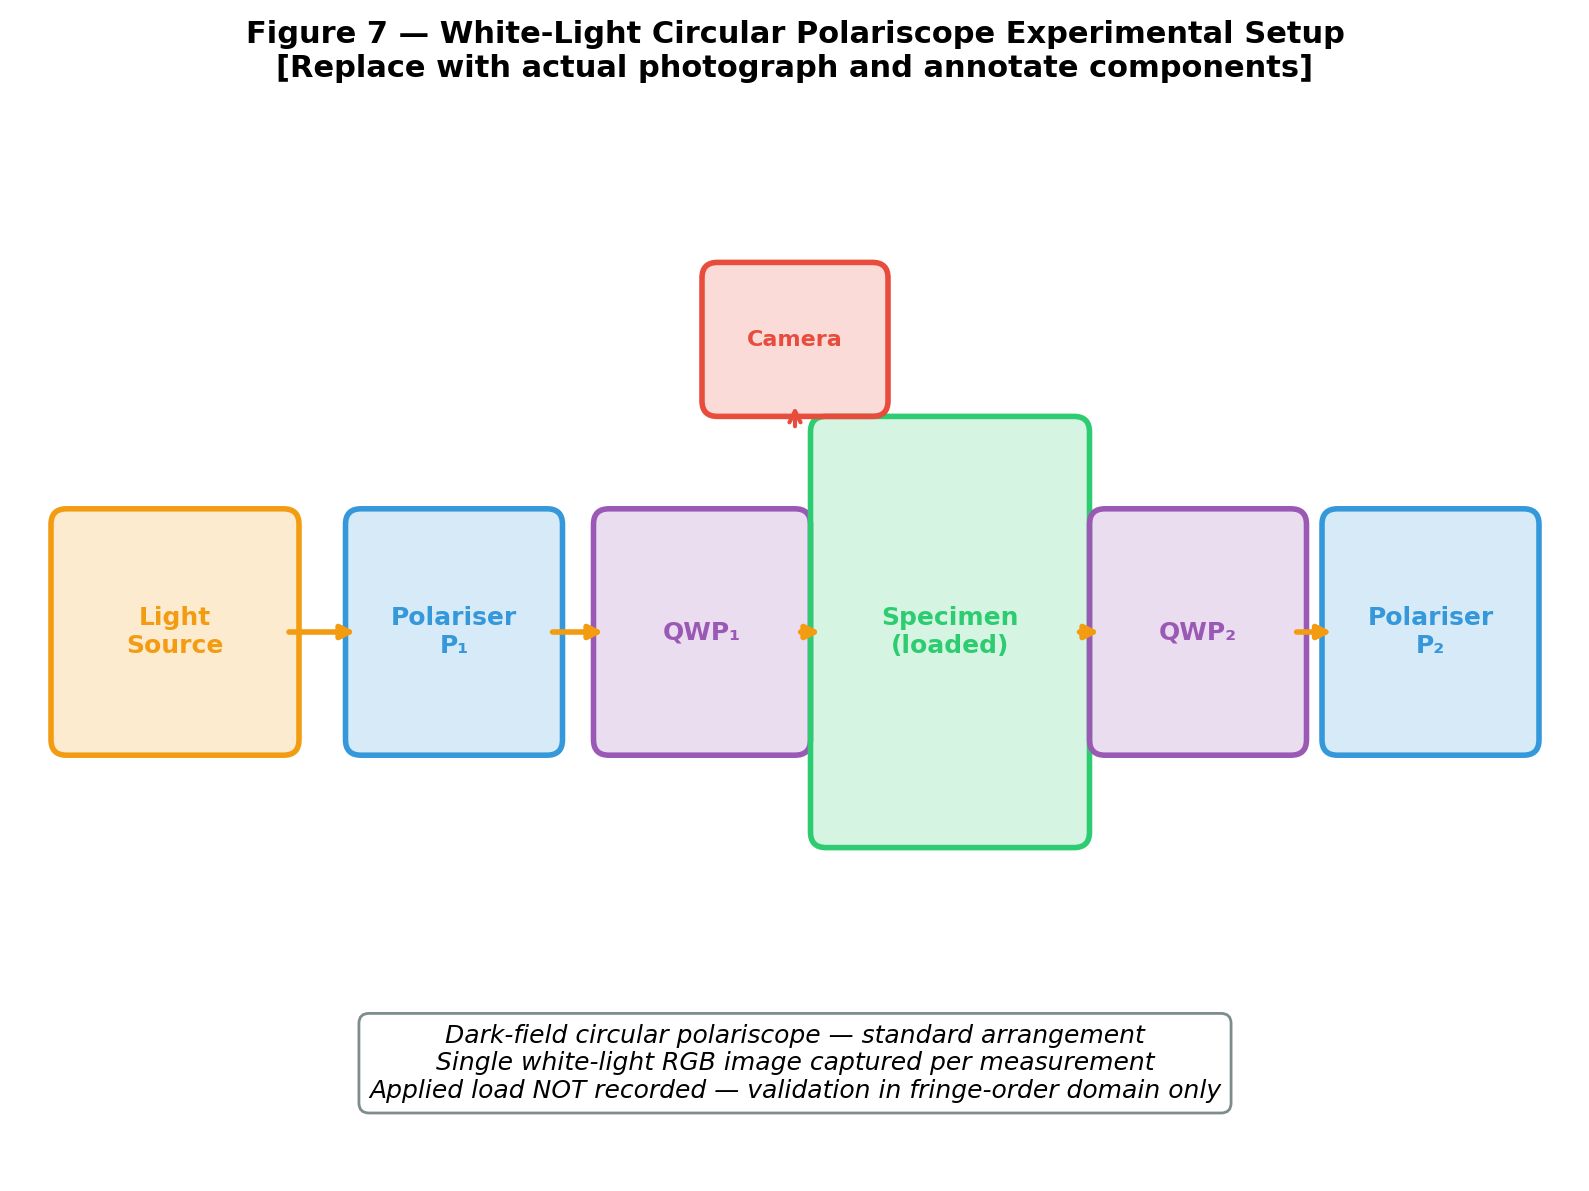
\includegraphics[width=0.72\linewidth]{Fig7_experimental_setup}
  \caption{White-light circular polariscope experimental setup.}
  \label{fig:setup}
\end{figure}

\subsection{Image Preprocessing and Normalisation}
\label{sec:preprocessing}

Before feature extraction, we mask and normalize each image. We use intensity thresholding and morphological erosion. This removes the inner hole and outer background from the evaluation metrics.

% ===========================================================
\section{Results}
\label{sec:results}

\subsection{Dataset Statistics}

The combined training dataset contained approximately 12.5~million pixel
rows across 570 synthetic and 280 real augmented images.
Table~\ref{tab:dataset_stats} provides the per-geometry and per-domain
breakdown.

\begin{table}[htbp]
  \centering
  \caption{Dataset statistics by geometry and domain after chunked
    train/test split.}
  \label{tab:dataset_stats}
  \small
  \begin{tabular}{@{}llccc@{}}
    \toprule
    Geometry / Source & Domain & Train rows & Test rows & \% of total \\
    \midrule
    Beam              & Synthetic      & 5\,666\,000 & 1\,623\,224 & 58.5\% \\
    Plate-with-hole   & Synthetic      &   897\,176  &   177\,904  &  8.6\% \\
    Disc              & Synthetic      &   436\,716  &   154\,296  &  4.7\% \\
    Real (7 types)    & Real-augmented & 2\,820\,000 &   680\,000  & 28.2\% \\
    \midrule
    Total             & ---            & 9\,819\,892 & 2\,635\,424 & 100\%  \\
    \bottomrule
  \end{tabular}
\end{table}

\subsection{Training Convergence}
\label{sec:convergence}

Both models trained smoothly. The training RMSE kept dropping over the $5{,}000$ rounds, and neither model stopped early. This shows that the models hadn't hit their performance ceiling at the $5{,}000$-round limit. So, the reported metrics are a conservative estimate of the method's potential accuracy. Boosting the round budget should lead to more improvement. It’s a key focus for future efforts. The lack of over-fitting shows that the test RMSE matches the training RMSE closely. This confirms that regularisation works well on the entire $70$~GB dataset.

\begin{figure}[htbp]
  \centering
  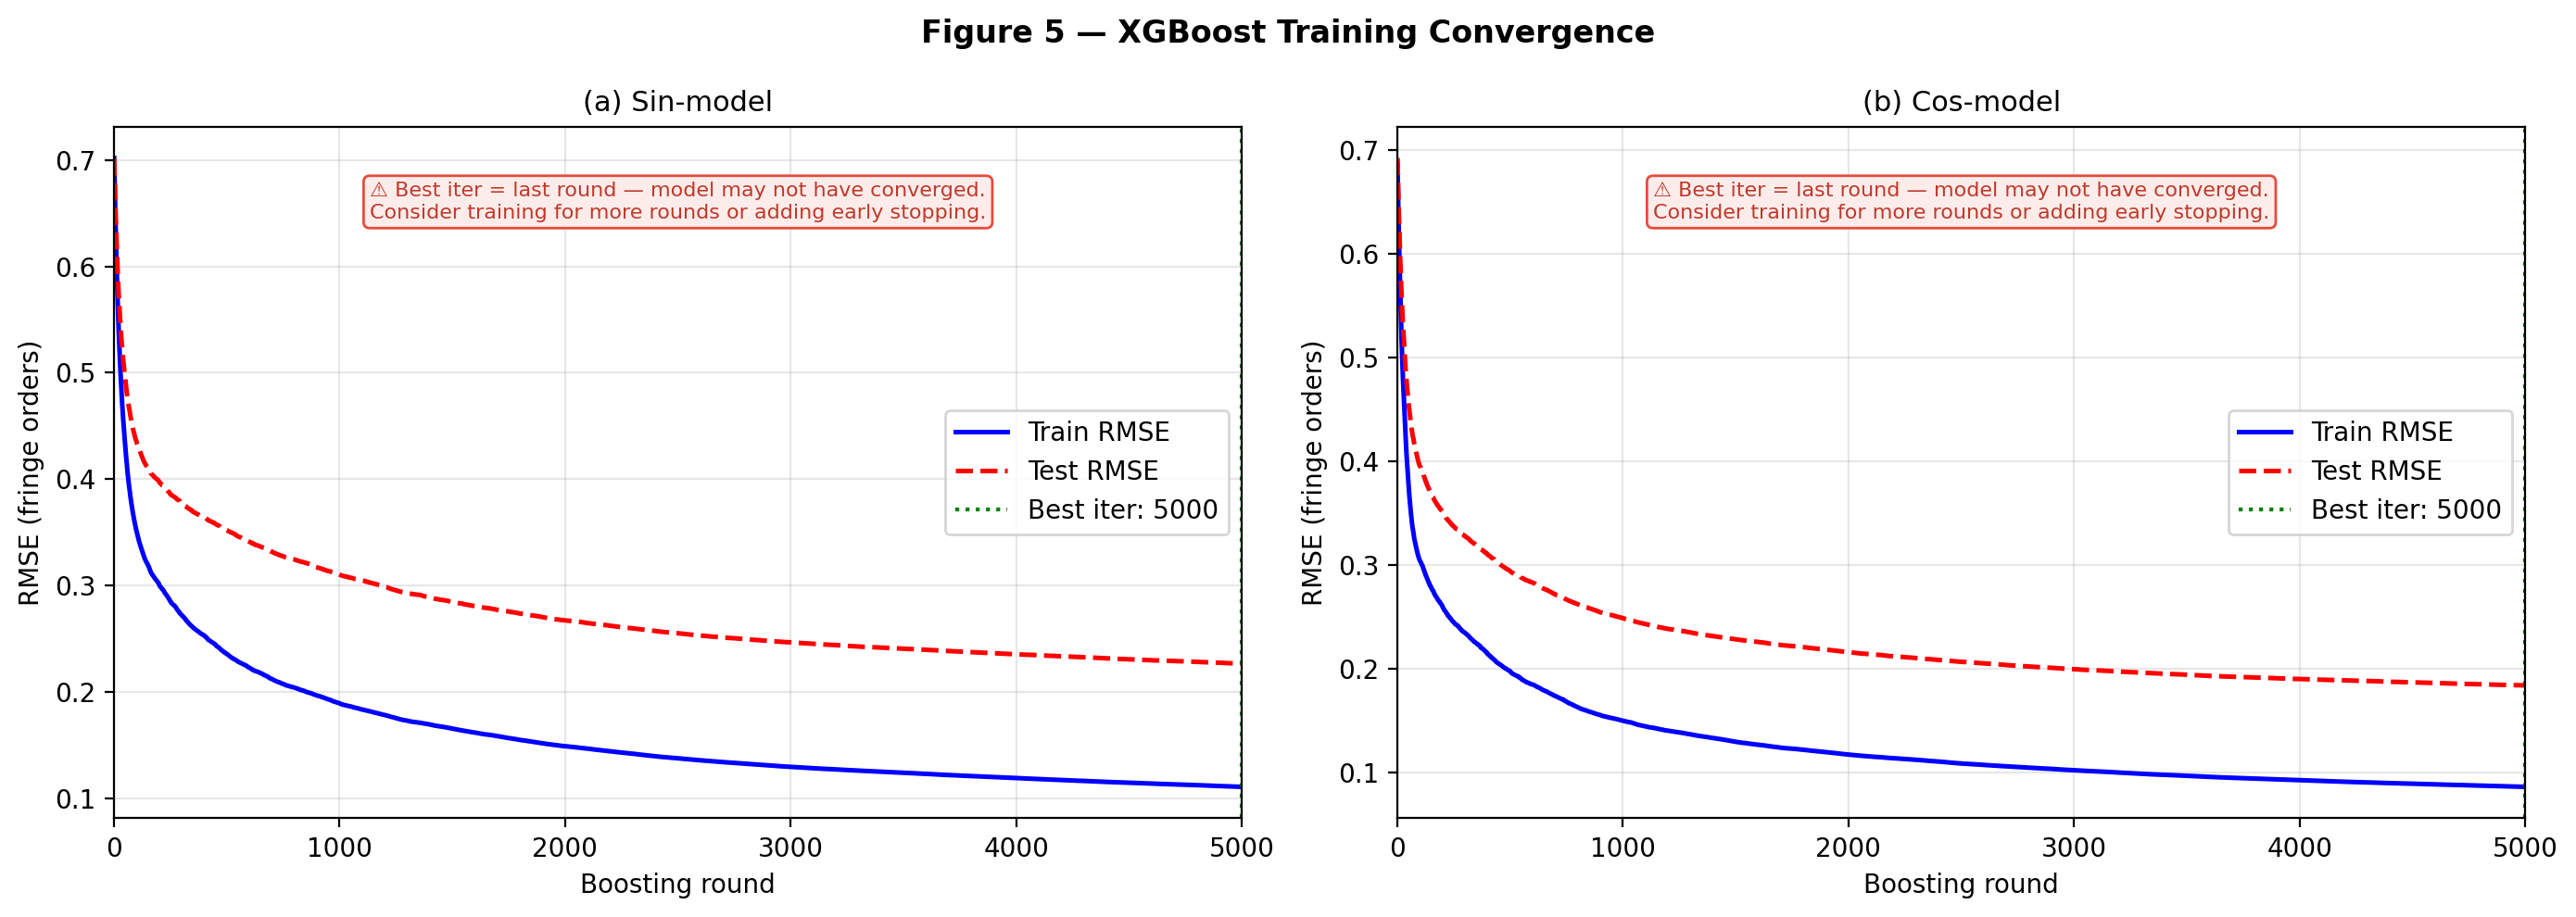
\includegraphics[width=0.96\linewidth]{Fig5_convergence}
  \caption{XGBoost training convergence. (a) Sin-model. (b) Cos-model.
    Solid line: training RMSE. Dashed line: held-out test RMSE (fringe
    orders). Both models reached the 5{,}000-round budget without
    triggering early stopping, indicating that reported metrics are
    conservative lower-bound estimates of achievable accuracy.}
  \label{fig:convergence}
\end{figure}

\subsection{Overall Prediction Performance on Synthetic Test Set}

Table~\ref{tab:overall_performance} summarises performance on the held-out
synthetic test set.

\begin{table}[htbp]
  \centering
  \caption{Overall fringe order prediction performance on the held-out
    synthetic test set. All metrics are conservative estimates; see
    Section~\ref{sec:convergence}.}
  \label{tab:overall_performance}
  \small
  \begin{tabular}{@{}lll@{}}
    \toprule
    Metric & Value & Note \\
    \midrule
    RMSE (fringe orders) & 0.1112 & Stress equiv.\ $\approx 0.224$~MPa (synthetic only) \\
    $R^2$                & 0.8485 & --- \\
    MAE (fringe orders)  & 0.0239 & --- \\
    P95 (fringe orders)  & 0.0525 & --- \\
    \bottomrule
  \end{tabular}
\end{table}

\subsection{Per-Geometry Breakdown}

\begin{table}[htbp]
  \centering
  \caption{Per-geometry fringe order prediction performance on the
    held-out synthetic test set. All metrics in fringe orders.}
  \label{tab:per_geometry}
  \small
  \begin{tabular}{@{}lccccc@{}}
    \toprule
    Geometry & Test samples & RMSE & $R^2$ & MAE & P95 \\
    \midrule
    Beam            & 1\,623\,224 & 0.0846 & 0.9113 & 0.0129 & 0.0180 \\
    Plate-with-hole &   177\,904  & 0.1062 & 0.8547 & 0.0206 & 0.0307 \\
    Disc            &   154\,296  & 0.0294 & 0.9632 & 0.0077 & 0.0211 \\
    Real (7 types)  &   680\,000  & 0.1590 & 0.6658 & 0.0523 & 0.1916 \\
    \midrule
    All             & 2\,635\,424 & 0.1112 & 0.8485 & 0.0239 & 0.0525 \\
    \bottomrule
  \end{tabular}
\end{table}

\begin{figure}[htbp]
  \centering
  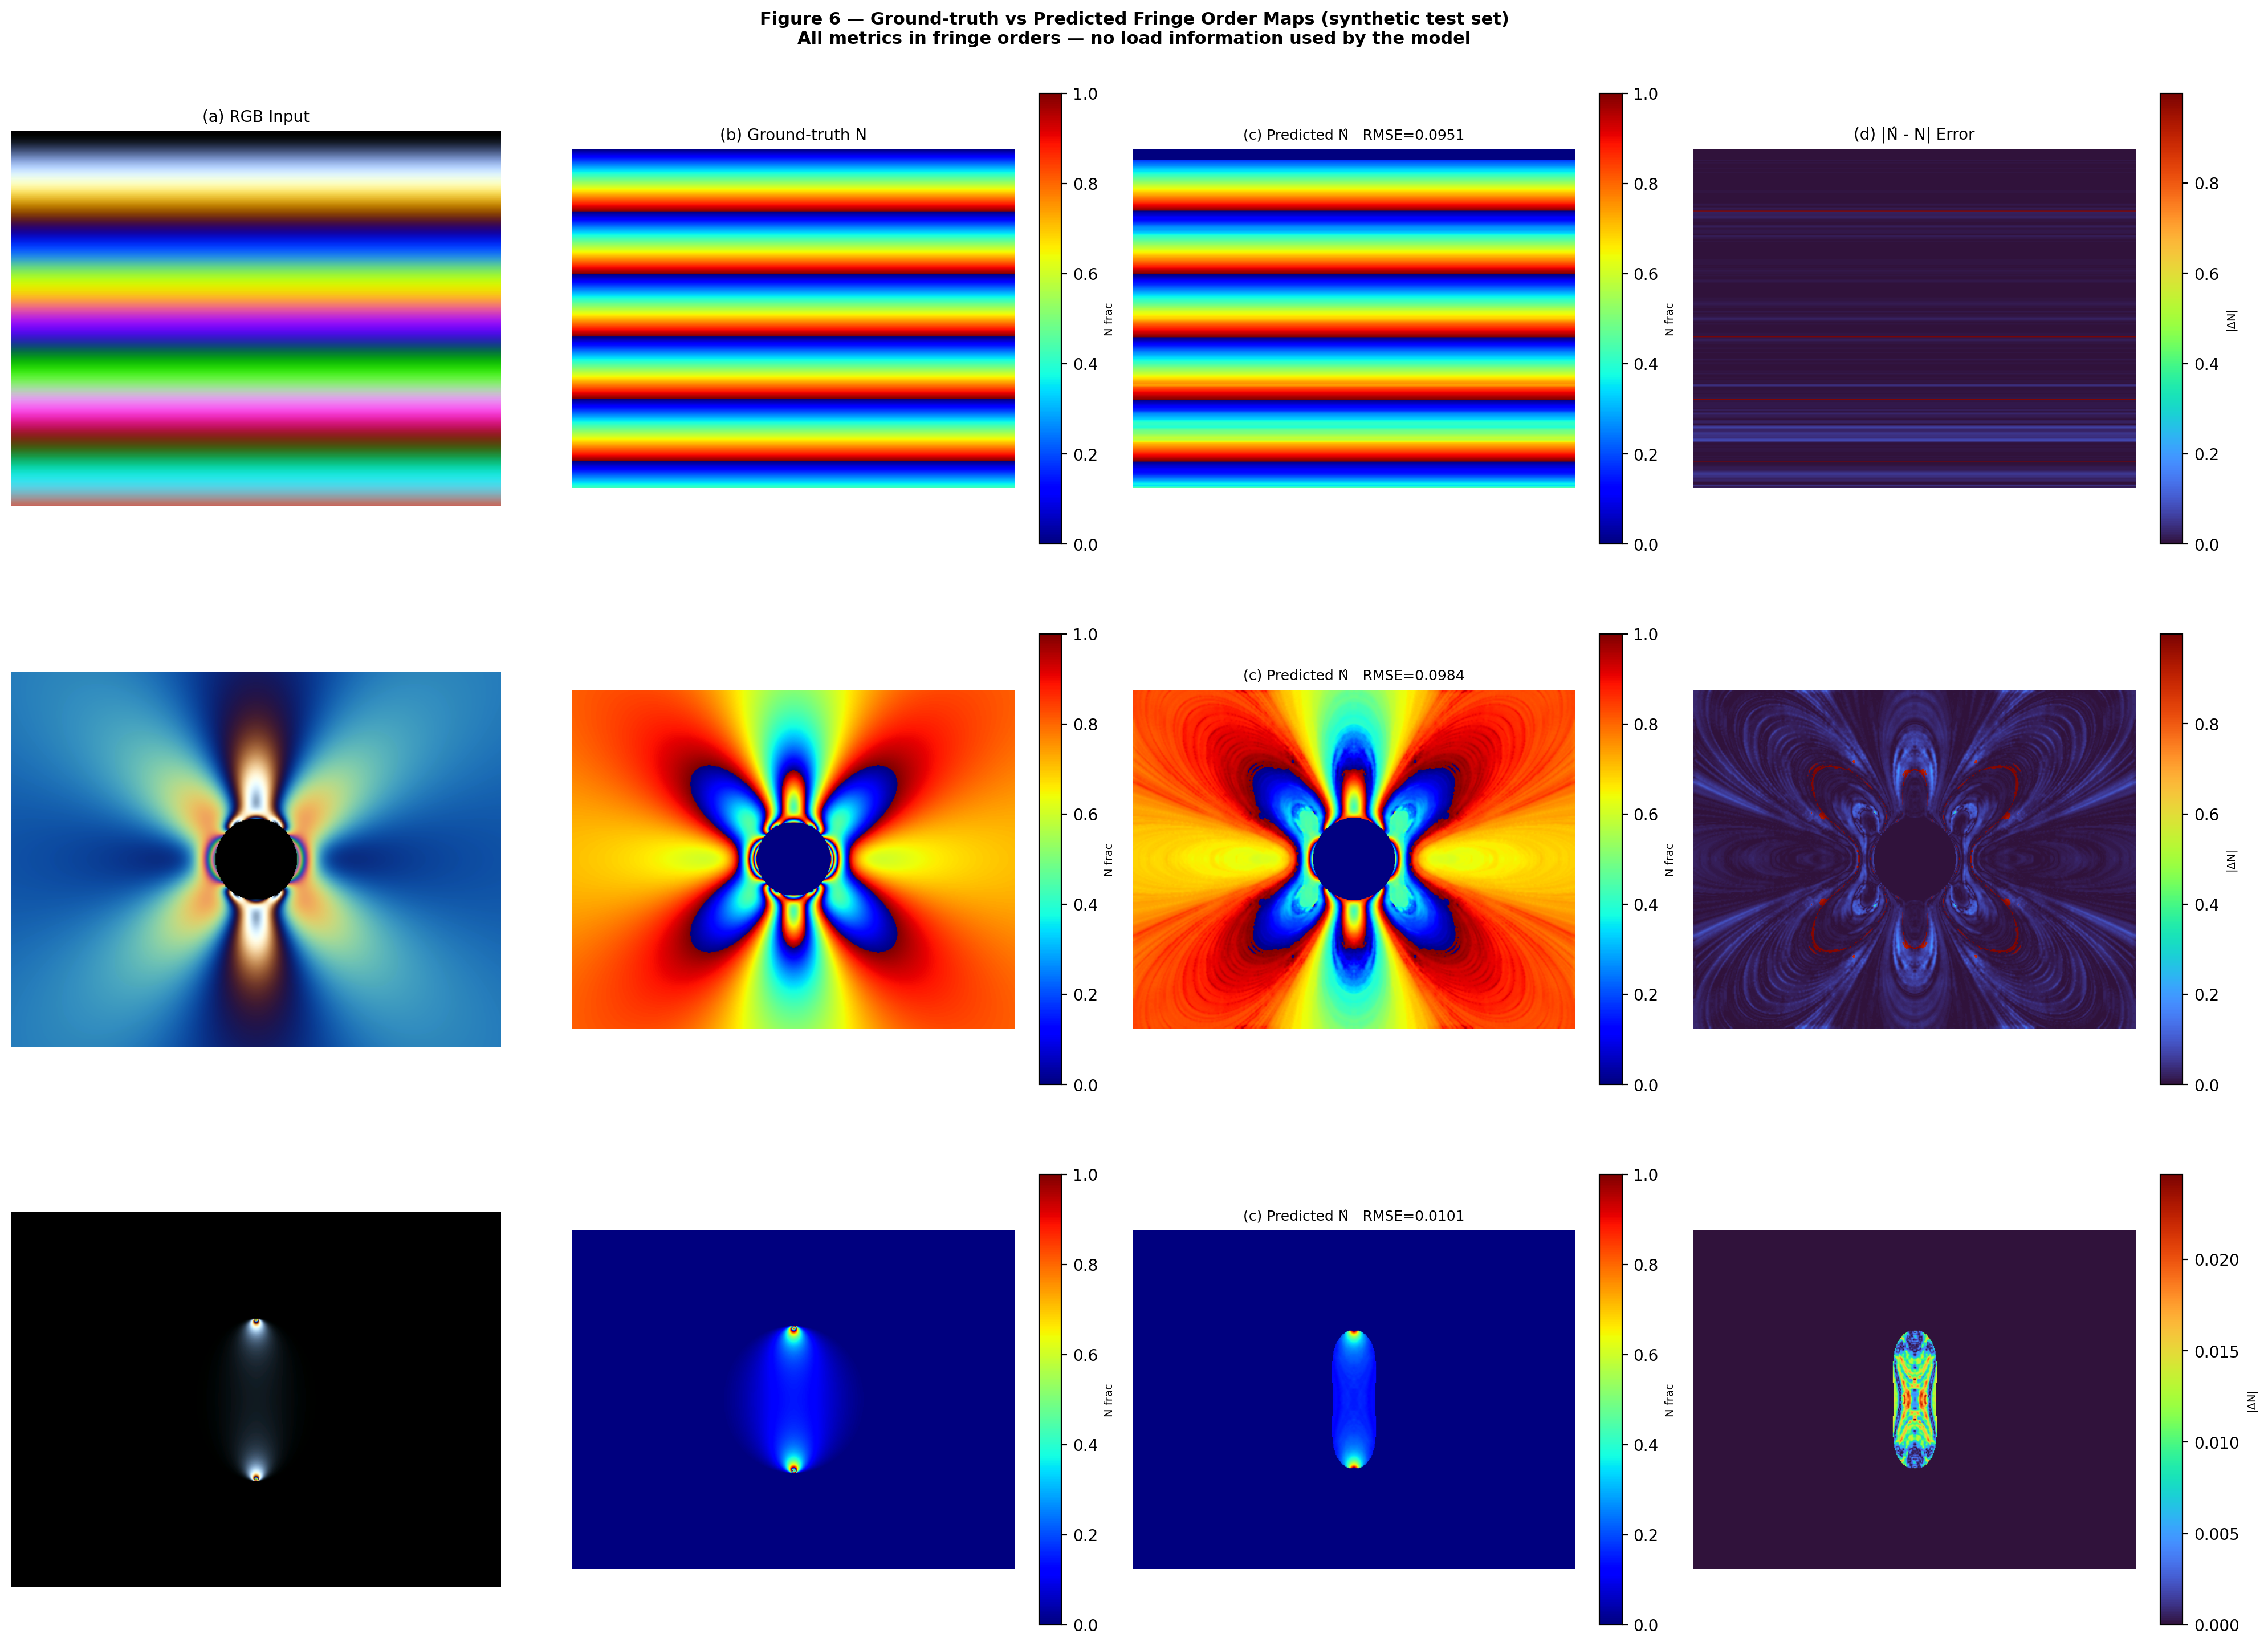
\includegraphics[width=0.96\linewidth]{Fig6_N_map_comparison}
  \caption{Ground-truth vs.\ predicted fringe order maps for representative
    synthetic test images. Columns: (a)~RGB input; (b)~ground-truth $N$ map;
    (c)~predicted $\hat{N}$ map with per-image RMSE; (d)~absolute pixel-wise
    error $|\hat{N}-N|$ in fringe orders.}
  \label{fig:n_maps}
\end{figure}

\subsection{Feature Importance}

The average gain-based feature importance for the sin-model and cos-model is shown in Fig.~6. The coarse Gabor filter at $45^\circ$ (\texttt{Gabor2\_45}, gain~267.7) is the top feature. Here are the circular hue encodings: \texttt{HueCos} at 173.3, \texttt{HueSin} at 156.9, and the normalized red channel, \texttt{R\_norm}, at 160.9. Colour-based features dominate texture features, following the physical model in Eq.~(4).

\begin{figure}[htbp]
  \centering
  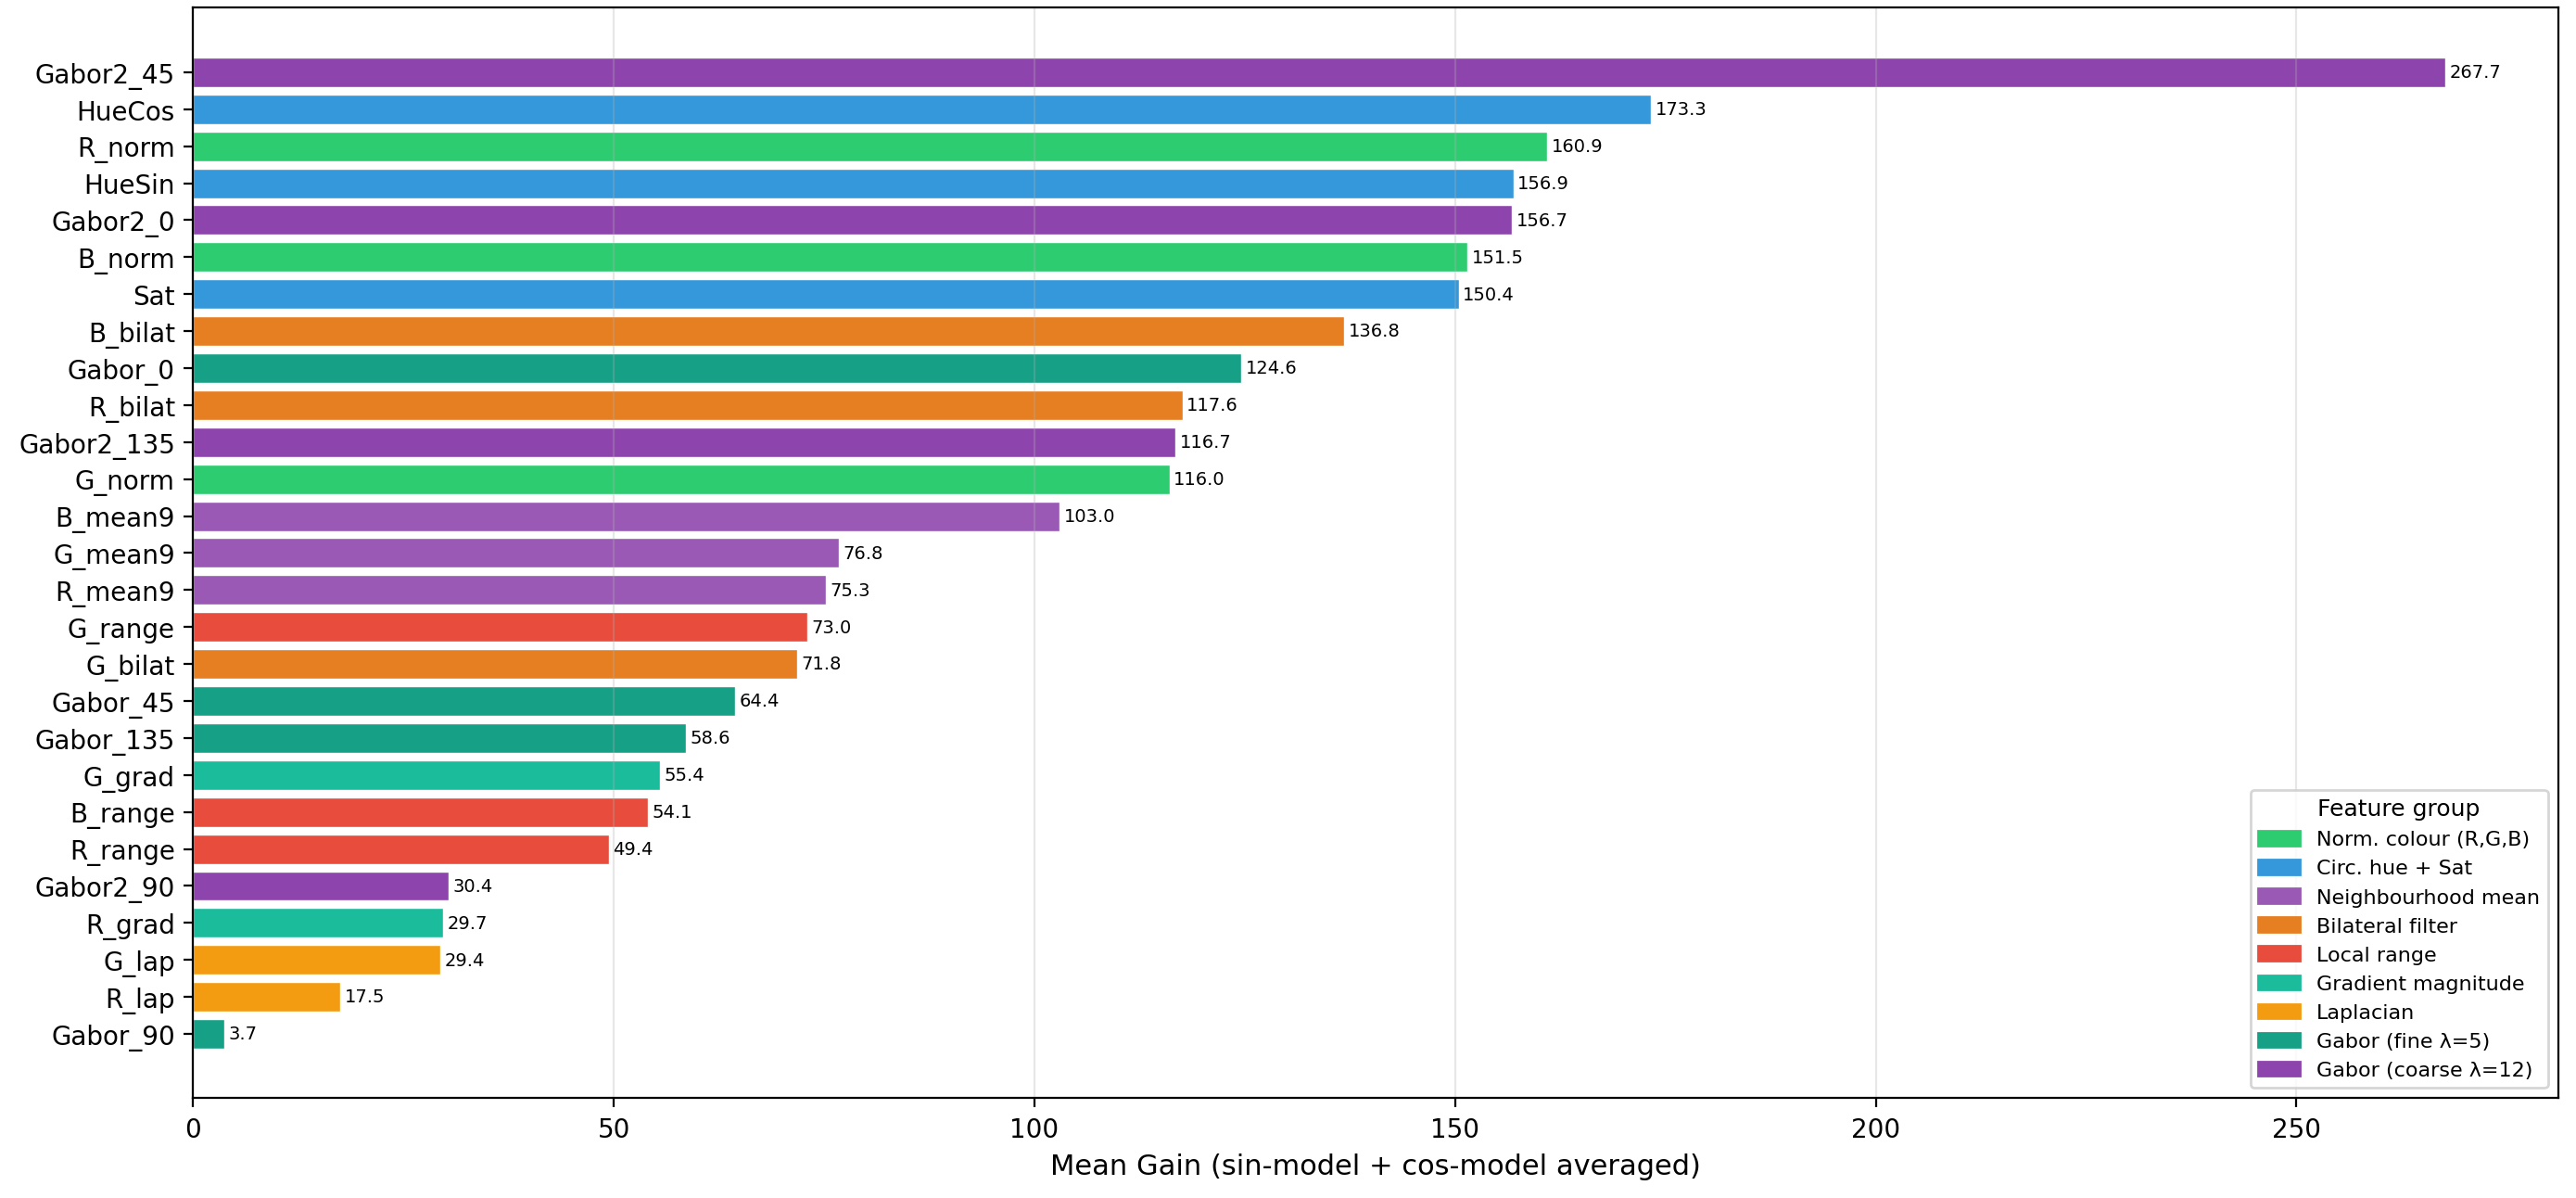
\includegraphics[width=0.94\linewidth]{Fig9_feature_importance}
  \caption{XGBoost feature importance (mean gain) averaged over sin-model
    and cos-model. All features are image-derived. The gain metric
    quantifies the average reduction in loss contributed by each feature
    across all splits in all trees.}
  \label{fig:feature_importance}
\end{figure}

\subsection{Validation on Unseen Experimental Specimens}

The trained model was applied to full-field prediction on ring and disc
experimental specimens not included in any stage of training.
Table~\ref{tab:experimental_results} reports quantitative performance.

\begin{table}[htbp]
  \centering
  \caption{Fringe order prediction performance on unseen experimental
    specimens. All metrics in fringe orders.}
  \label{tab:experimental_results}
  \small
  \begin{tabular}{@{}lcccc@{}}
    \toprule
    Specimen & Pixels evaluated & RMSE & $R^2$ & MAE \\
    \midrule
    Ring & 164\,458 & 0.4912 & 0.7575 & 0.2837 \\
    Disc & 205\,695 & 0.2301 & 0.9609 & 0.0529 \\
    \bottomrule
  \end{tabular}
\end{table}

\begin{figure}[htbp]
  \centering
  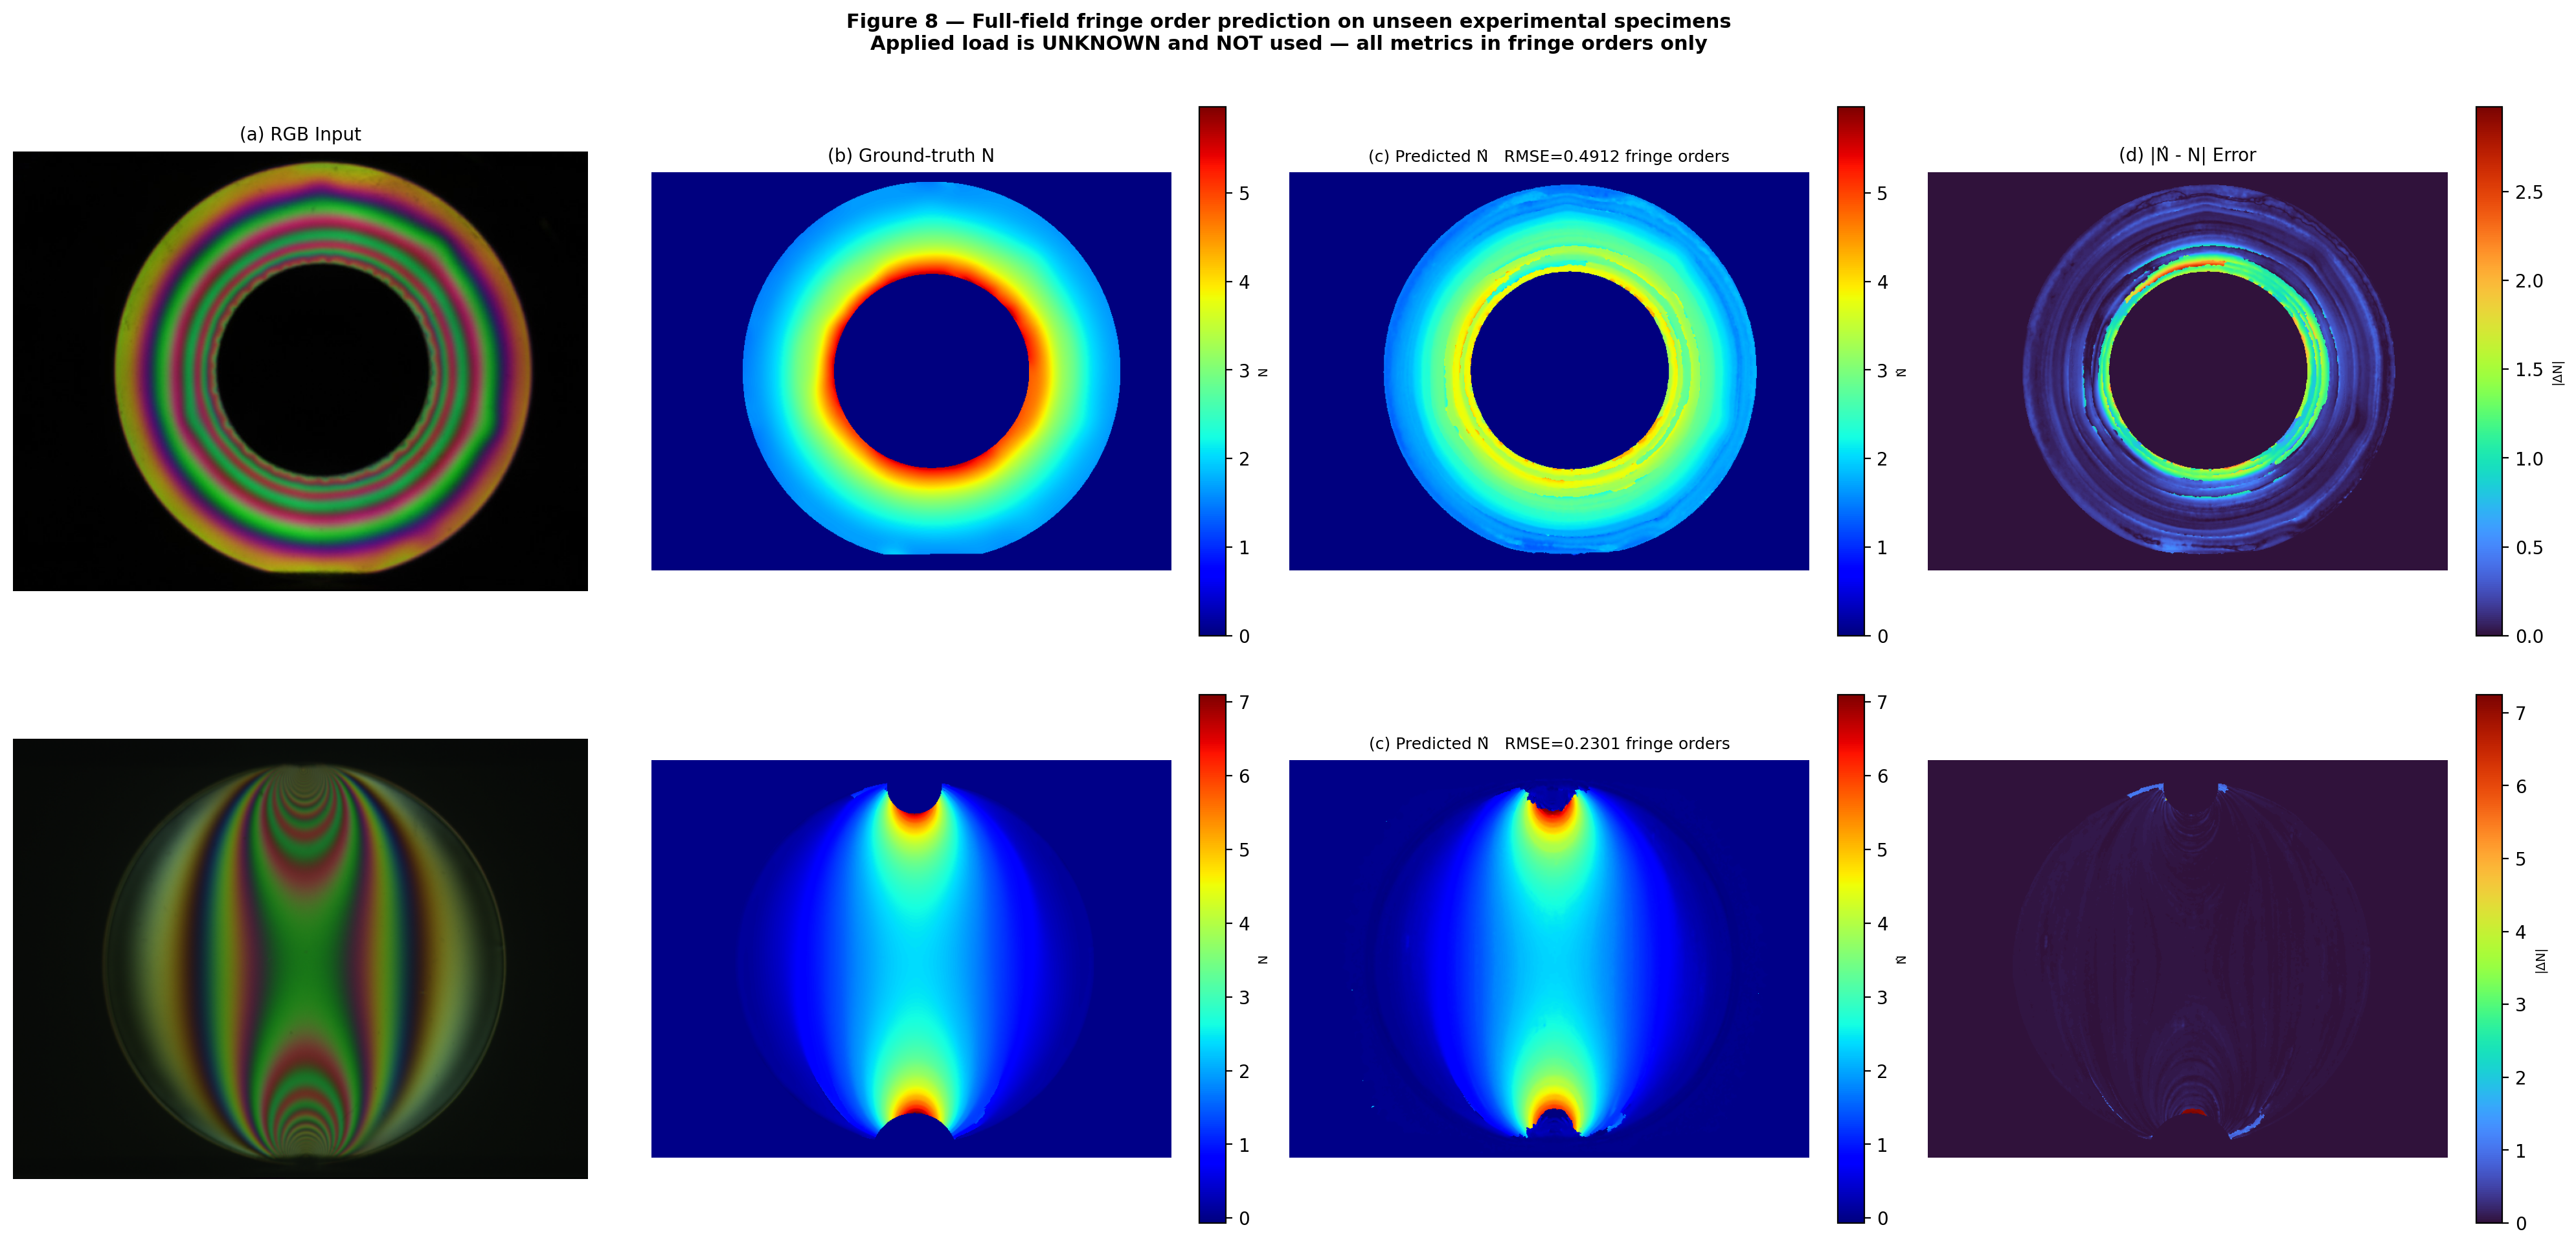
\includegraphics[width=0.96\linewidth]{Fig8_experimental_validation}
  \caption{Full-field fringe order prediction on unseen experimental specimens.
    (a)--(d) Ring specimen. (e)--(h) Disc specimen. All error maps are in
    fringe orders.}
  \label{fig:experimental_validation}
\end{figure}

\subsubsection{Detailed Analysis: Ring Specimen}
\label{sec:ring_detail}

Fig.~\ref{fig:ring_best_result} presents the complete best-result analysis
for the ring specimen under the optimal inference hyperparameters
(global normalisation, $\sigma = 2.0$, erosion disk~$= 7$, blend
weight~$= 1.0$), selected by the automated grid search
(Section~\ref{sec:hyperparameter_sweep}).

\begin{figure}[htbp]
  \centering
  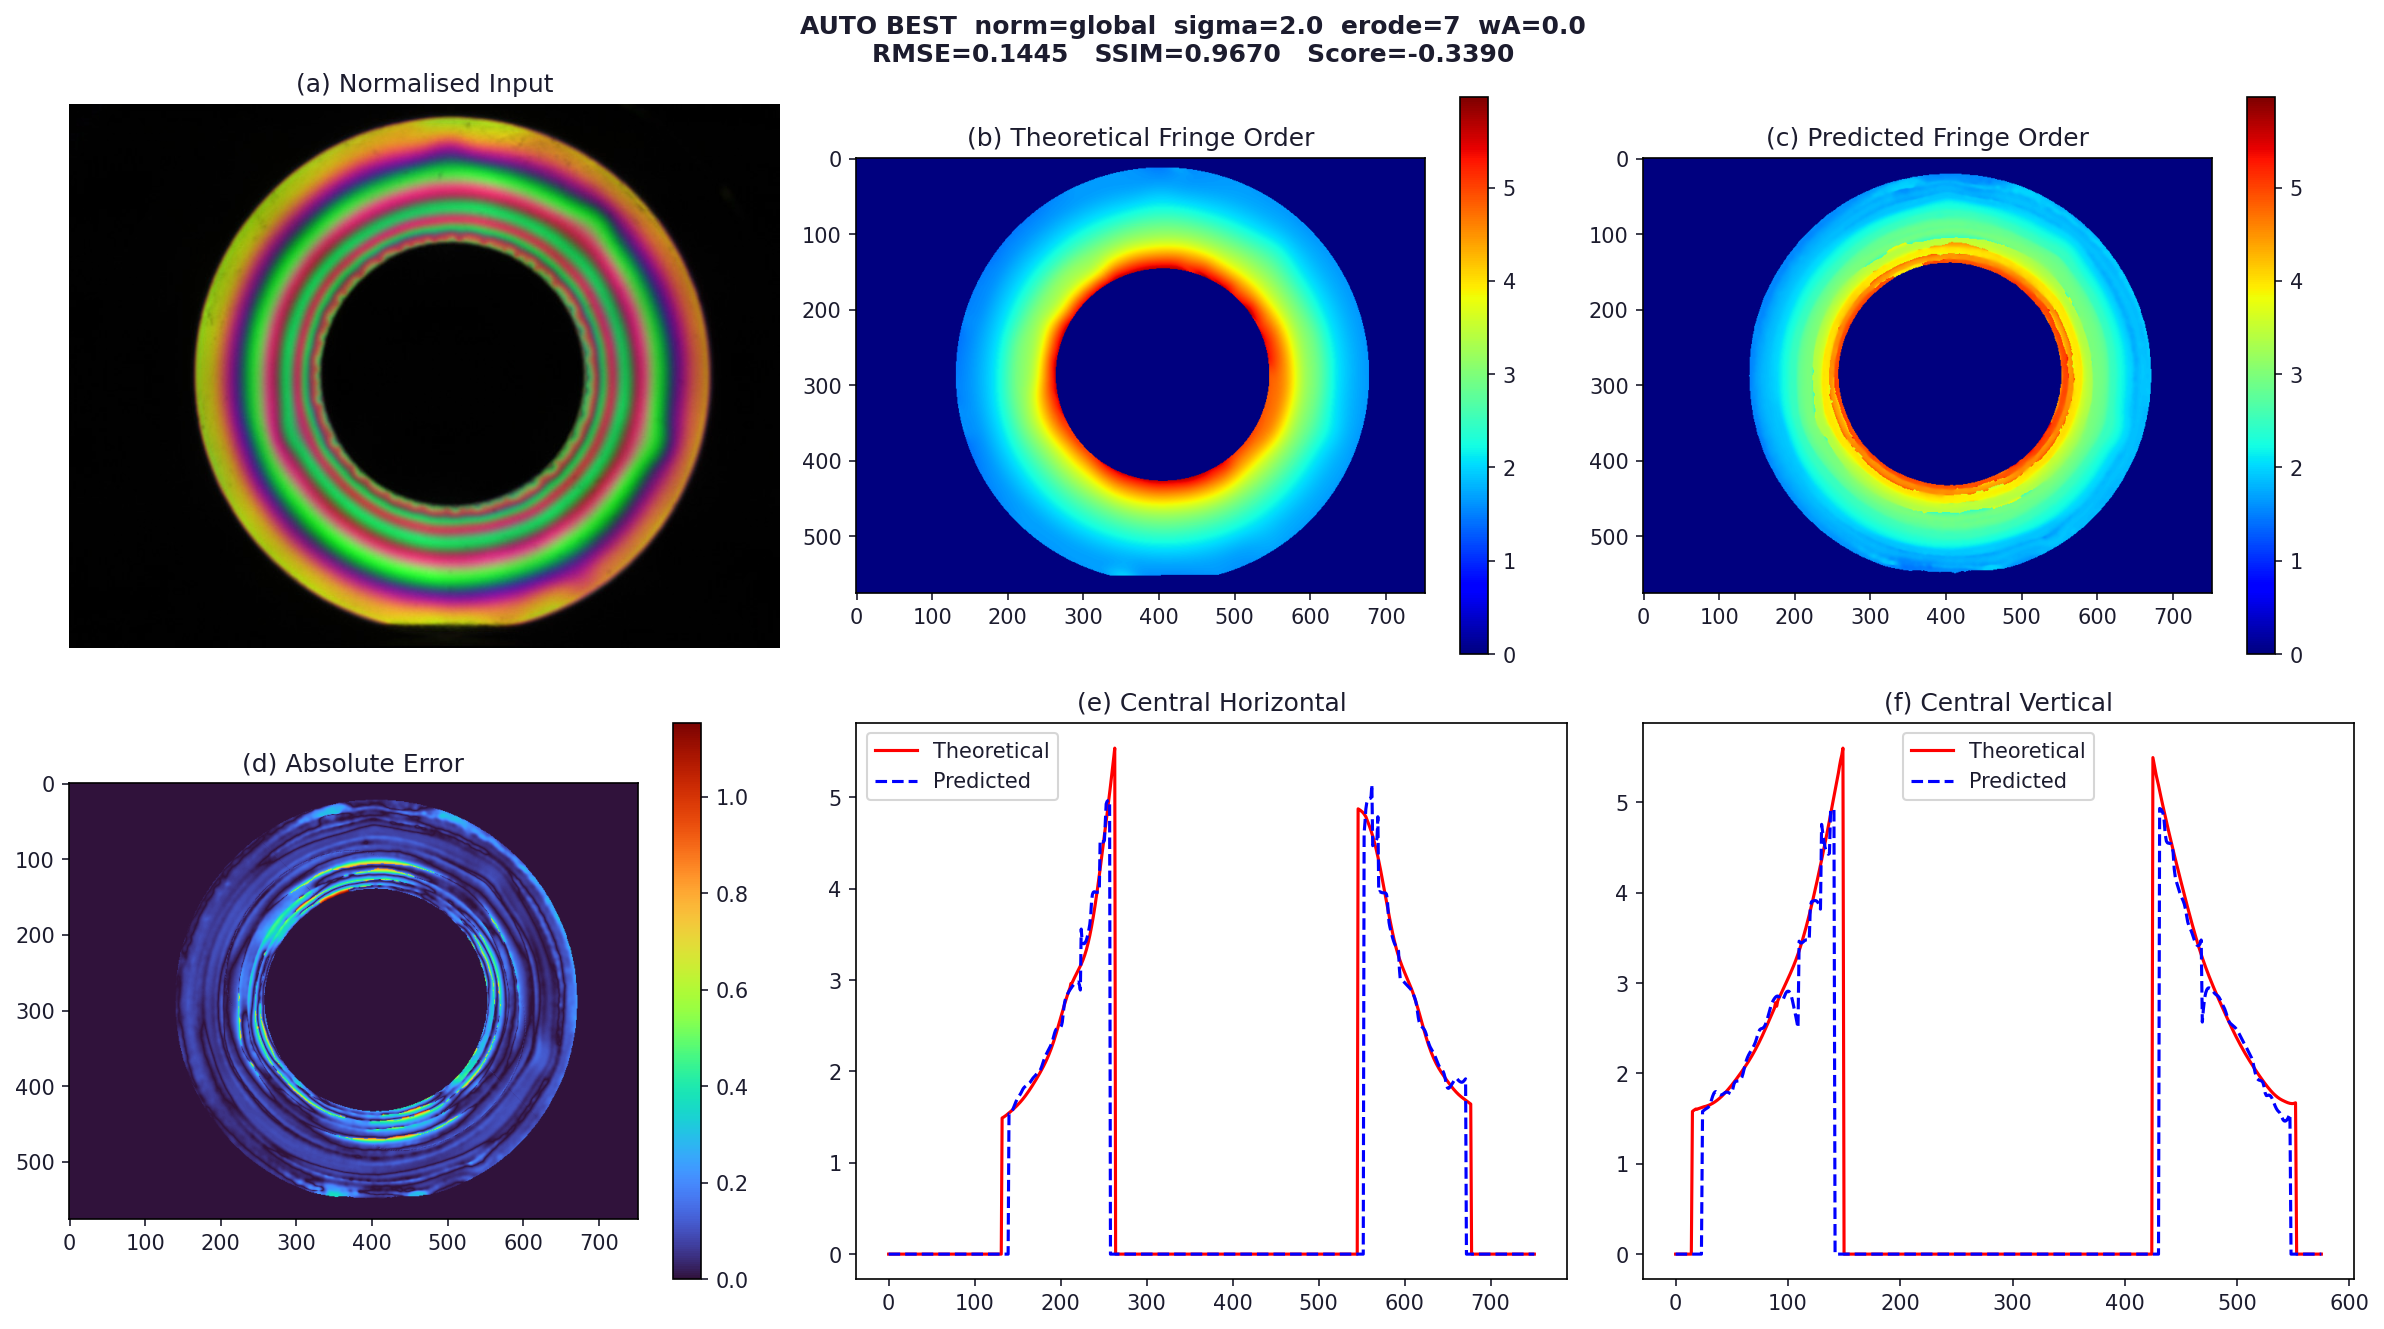
\includegraphics[width=0.98\linewidth]{auto_best_result}
  \caption{Best-result analysis for the ring specimen.
    (a)~Normalised input image. (b)~Theoretical fringe order $N$.
    (c)~Predicted $\hat{N}$. (d)~Absolute error $|\hat{N}-N|$.
    (e)~Central horizontal profile: theoretical (red solid) vs.\ predicted
    (blue dashed). (f)~Central vertical profile.
    Best inference parameters: global normalisation, $\sigma{=}2.0$,
    erosion disk~$= 7$, $\mathrm{RMSE} = 0.1445$, $\mathrm{SSIM} = 0.9670$.}
  \label{fig:ring_best_result}
\end{figure}

\begin{figure}[htbp]
  \centering
  \begin{minipage}[t]{0.32\linewidth}
    \centering
    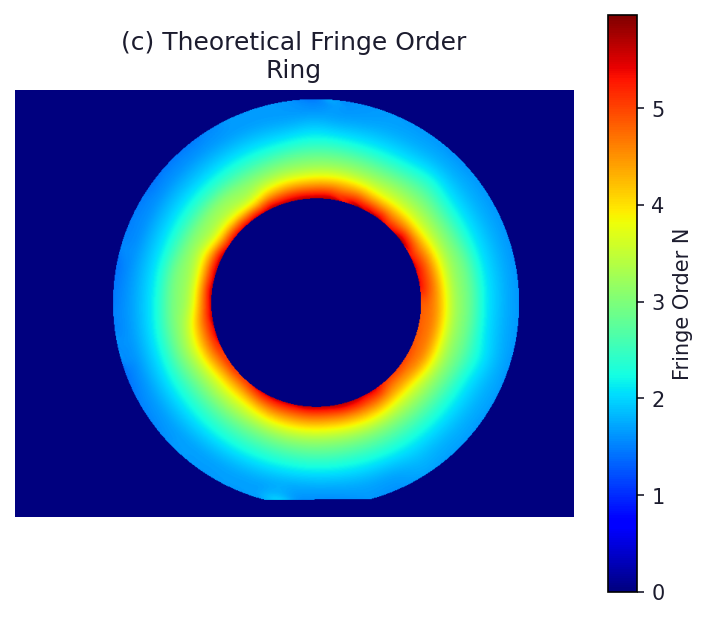
\includegraphics[width=\linewidth]{ind_c_theoretical_fringe}
    \caption{Theoretical fringe order $N$ for the ring specimen.}
    \label{fig:ring_gt}
  \end{minipage}\hfill
  \begin{minipage}[t]{0.32\linewidth}
    \centering
    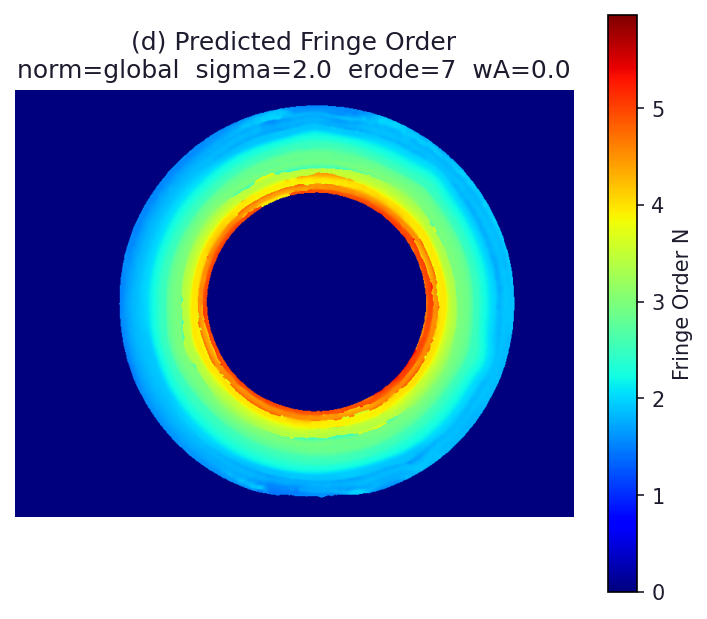
\includegraphics[width=\linewidth]{ind_d_predicted_fringe}
    \caption{Predicted $\hat{N}$ for the ring specimen.}
    \label{fig:ring_pred}
  \end{minipage}\hfill
  \begin{minipage}[t]{0.32\linewidth}
    \centering
    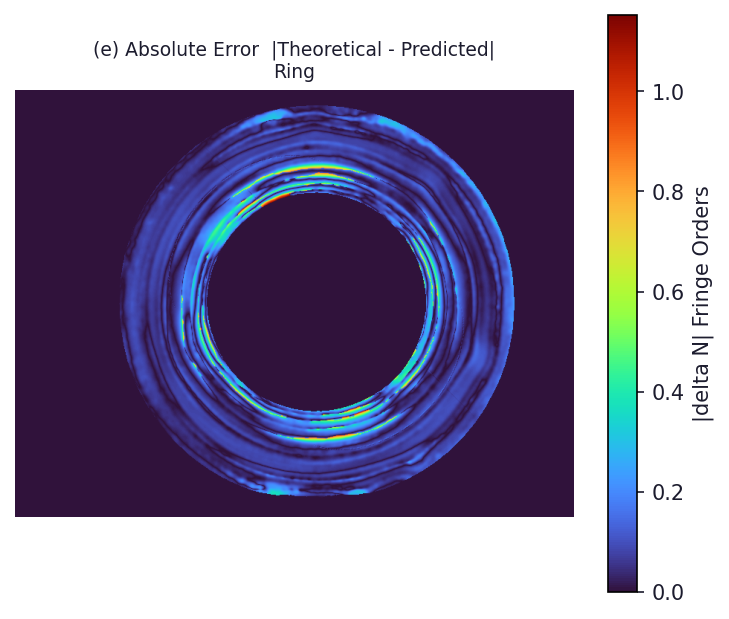
\includegraphics[width=\linewidth]{ind_e_absolute_error}
    \caption{Absolute error $|\hat{N}-N|$ for the ring specimen.}
    \label{fig:ring_error}
  \end{minipage}
\end{figure}

\begin{figure}[htbp]
  \centering
  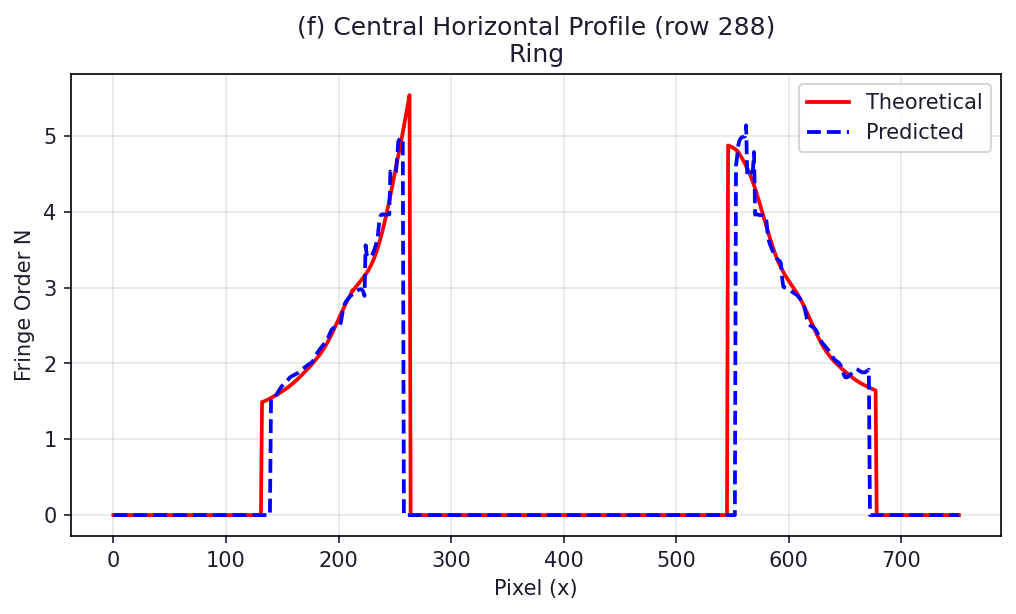
\includegraphics[width=0.49\linewidth]{ind_f_profile_horizontal}
  \hfill
  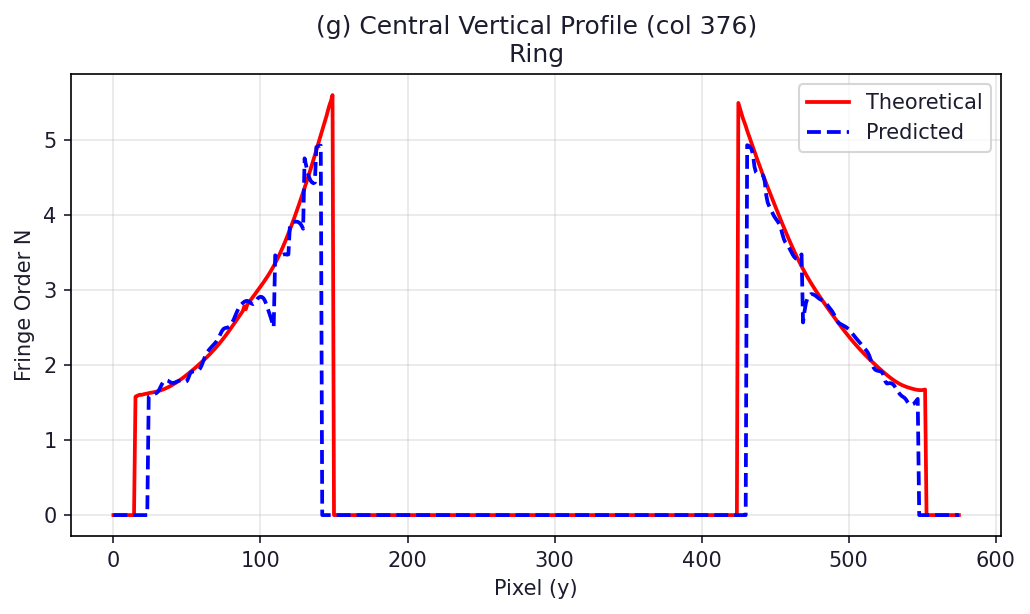
\includegraphics[width=0.49\linewidth]{ind_g_profile_vertical}
  \caption{Central line profiles for the ring specimen. Left: horizontal
    profile (row~288). Right: vertical profile (col~376). Red solid:
    theoretical $N$. Blue dashed: predicted $\hat{N}$.}
  \label{fig:ring_profiles}
\end{figure}

% ===========================================================
\section{Discussion}
\label{sec:discussion}

\subsection{Accuracy and Physical Interpretation}

The overall RMSE of 0.1112 fringe orders on the synthetic test set
corresponds to a principal stress difference uncertainty of approximately
0.224~MPa (Eq.~\ref{eq:stress_uncertainty}, $h=6$~mm,
$C=4.55\times10^{-11}$~m$^2$/N). For context, TFP with advancing-front
refinement achieves RMSE~$\approx 0.02$--$0.05$ fringe orders in
well-resolved regions \cite{madhu2007,kale2013}, and phase-stepping methods
achieve sub-0.01 fringe orders under controlled conditions
\cite{wang1995,siegmann2005}. The present ML approach falls between standard
TFP and scanning-refined TFP accuracy in smooth fringe regions. The reported
metrics are conservative lower bounds, as training had not yet converged at
the 5{,}000-round budget (Section~\ref{sec:convergence}).

The sin/cos encoding (Eqs.~\eqref{eq:encoding}--\eqref{eq:recovery})
completely eliminated the integer wrap-around artefacts observed in
preliminary scalar regression experiments, confirming resolution of the
circular discontinuity without a spatial continuity penalty in the loss
function \cite{mohan2024,ramesh2008}. The quality metric $\varepsilon$
provides a natural per-pixel uncertainty estimate without additional
computation.

The gain-based feature importance (Fig.~\ref{fig:feature_importance}) shows
that \texttt{Gabor2\_45} (mean gain~267.7) is the single most discriminating
feature, followed by circular hue encoding and normalised colour. This is
physically interpretable: the coarse Gabor at $45^\circ$ captures the
diagonal fringe texture characteristic of the isochromatic pattern, while
hue encoding directly reflects the spectral signature encoded in
Eq.~\eqref{eq:camera}.

\subsection{Ring Specimen Performance}

The ring specimen RMSE of 0.4912 fringe orders is substantially higher than
the disc result (0.2301), and warrants explicit discussion. The error map
(Fig.~\ref{fig:ring_error}) reveals that high errors are concentrated along
the inner and outer ring boundaries---regions of steep $|\nabla N|$. The
pixel-wise model has no spatial continuity constraint, so it cannot
propagate context across sharp fringe gradients. This is a structural
limitation of the current approach rather than a generalisation failure: the
smooth interior region of the ring achieves low error (RMSE~$= 0.1445$
under optimal inference parameters, SSIM~$= 0.9670$, Fig.~\ref{fig:ring_best_result}),
comparable to the disc result.

Two factors compound the boundary error. First, the ground-truth phase-stepped
$N$ map for the ring specimen also contains higher uncertainty near the inner
boundary due to steep fringe gradients. Second, the ring geometry---with its
concentric high-gradient annular fringe bands---differs substantially from
any geometry in the synthetic training set, limiting the representativeness
of learned boundary features. Integration with quality-guided phase
unwrapping \cite{ramji2010,ramesh2004}, using the $\varepsilon$ confidence
metric to down-weight boundary pixels, is anticipated to substantially
reduce this error.

\subsection{Comparison with Existing Methods}

Table~\ref{tab:comparison} places the proposed method alongside
representative demodulation approaches. The proposed method requires no
material-specific calibration specimen or LUT, no motorised retarder, and
only a single image. It provides direct physical interpretability through
gain-based feature importance, which distinguishes it from deep learning
approaches such as FringeNet \cite{mohan2024} where saliency maps are
required as a post-hoc approximation. A quantitative comparison with
FringeNet on a common benchmark dataset is not presented here because the
Isochromatic-Art dataset \cite{mohan2024} employs a different specimen
set, spectral rendering pipeline, and evaluation protocol from the present
work; such a comparison on a unified benchmark is identified as important
future work.

\begin{table}[htbp]
  \centering
  \caption{Comparison of fringe order demodulation methods. Calibration
    refers to a material-specific LUT or calibration specimen.}
  \label{tab:comparison}
  \footnotesize
  \begin{tabular}{@{}lccccL{2.2cm}l@{}}
    \toprule
    Method & Images & Extra HW & Calibration & Interpretable & Approx.\ RMSE & Ref. \\
    \midrule
    RGB TFP (original)   & 1      & No  & Yes (LUT) & No
      & 0.05--0.15 & \cite{ajovalasit1995,ramesh1996} \\
    TFP $+$ scanning     & 1      & No  & Yes (LUT) & No
      & 0.02--0.05 & \cite{madhu2007,kale2013} \\
    Phase-stepping (6-step) & $\ge 6$ & Yes & No     & No
      & ${<}0.01$  & \cite{wang1995,siegmann2005,ramesh1996phaseshifting} \\
    Fourier transform    & 1      & No  & No        & No
      & 0.05--0.10 & \cite{quan1993,morimoto1994} \\
    FringeNet (U-Net)    & 1      & No  & No        & Partial
      & Not directly comparable$^\dagger$ & \cite{mohan2024} \\
    Proposed (XGBoost)   & 1      & No  & No        & Yes (gain)
      & 0.11 (conservative)  & This work \\
    \bottomrule
  \end{tabular}
  \vspace{2pt}\\
  \footnotesize $^\dagger$ FringeNet results are reported on the
  Isochromatic-Art benchmark using a different specimen set and evaluation
  protocol; a direct numerical comparison requires evaluation on a common
  dataset, identified as future work.
\end{table}

\subsection{Inference Hyperparameter Selection}
\label{sec:hyperparameter_sweep}

At inference time, three post-processing hyperparameters affect the final
predicted $\hat{N}$ map: the normalisation mode (per-channel or global),
the Gaussian smoothing $\sigma$ applied to the sin/cos maps before
$\mathrm{arctan2}$ recovery, and the morphological erosion disk radius.
An automated grid search over $2 \times 4 \times 3 = 24$ combinations was
performed, selecting the combination that minimises
$\mathrm{RMSE} - 0.5 \times \mathrm{SSIM}$. The optimal combination---
$\sigma = 2.0$, erosion disk~$= 7$---achieves RMSE~$= 0.1445$ fringe
orders and SSIM~$= 0.9670$.

\subsection{Limitations}

Four limitations should be noted. First, the model predicts fractional
fringe order only; integer-order recovery requires a phase-unwrapping step
\cite{ramesh2004,ramji2008}. Second, the pixel-wise model imposes no
spatial continuity across predictions; CNN or CRF post-processing is
expected to reduce boundary errors \cite{mohan2024,brinezdeleon2024}.
Third, the synthetic training set covers three analytical geometries;
specimens with complex three-dimensional stress states or FEM-required
boundary conditions were not included. Fourth, both models reached the
5{,}000-round training budget without converging; all reported metrics
are therefore conservative, and increased training rounds are expected to
improve performance.

\subsection{Future Work}

Future directions include: (i) extended training beyond 5{,}000 rounds to
reach full convergence; (ii) integration with quality-guided phase-unwrapping
\cite{ramji2010,ramesh2004} using the $\varepsilon$ confidence map;
(iii) FEM-based synthetic data generation for complex geometries;
(iv) domain adaptation for improved illumination robustness
\cite{brinezdeleon2024}; (v) evaluation on the Isochromatic-Art benchmark
\cite{mohan2024} for a direct comparison with FringeNet; and (vi) ablation
studies quantifying the contribution of individual feature groups and the
sin/cos encoding.

% ===========================================================
\section{Conclusion}
\label{sec:conclusion}

This paper presented a whole-field fringe order demodulation method for
digital photoelasticity based on dual XGBoost regression of
trigonometrically encoded targets. The key design principle is inference
from image features alone: a 27-dimensional pixel-level descriptor---
encoding normalised colour, circular hue, saturation, neighbourhood
statistics, bilateral filter responses, gradient, Laplacian, and
multi-scale Gabor filter outputs---is computed from the RGB image, with no
access to applied load, specimen geometry, or material constants at inference
time.

The sin/cos dual-target encoding cleanly resolves the circular discontinuity
at integer fringe orders, eliminating wrap-around artefacts without requiring
a spatial continuity penalty in the loss function. Physics-based analytical
solutions are used exclusively in the data generation phase to produce
synthetic fringe images across three specimen geometries and ten spectral
conditions; load values are not features of the trained model.

GPU-accelerated XGBoost processed the ${>}70$~GB dataset in memory-efficient
500k-row chunks. Experimental validation on unseen ring and disc specimens
demonstrated RMSE~$= 0.1112$ fringe orders ($R^2 = 0.8485$) on the
held-out synthetic test set, and RMSE~$= 0.2301$ fringe orders
($R^2 = 0.9609$) on the disc experimental specimen. These figures represent
conservative lower bounds, as training had not yet converged at the
5{,}000-round budget. The gain-based feature importance ranking provides
direct physical insight, with colour and orientation features dominating,
consistent with the underlying spectral physics of isochromatic fringe
formation. Future integration with quality-guided phase-unwrapping will
extend the method to absolute fringe order maps.

% ===========================================================
\section*{Acknowledgements}

[Acknowledge supervisor, institution, funding body, laboratory support, and
any computational resources used here.]

% ===========================================================
\section*{CRediT Author Contribution Statement}

[Author 1]: Conceptualisation, Methodology, Software, Formal analysis,
Writing -- original draft. [Author 2]: Supervision, Writing -- review \&
editing, Resources.

% ===========================================================
\section*{Declaration of Competing Interests}

The authors declare that they have no known competing financial interests or
personal relationships that could have appeared to influence the work
reported in this paper.

% ===========================================================
\section*{Data Availability Statement}

The source code for the complete pipeline (\texttt{generate\_dataset.py},
\texttt{augmentation.py}, \texttt{processing\_pipeline\_better.py},
\texttt{Trainer\_better.py}, and \texttt{Tester.py}) and the synthetic
dataset generation scripts are available at [repository URL]. The real
experimental image dataset will be made available upon reasonable request
to the corresponding author.

% ===========================================================
\bibliographystyle{elsarticle-num}
\bibliography{references}

% ===========================================================
\appendix

\section{Material and Optical Constants}
\label{app:constants}

\begin{table}[htbp]
  \centering
  \caption{Material and optical constants used in synthetic image generation.
    These constants are used only during data generation.}
  \label{tab:constants}
  \small
  \begin{tabular}{@{}L{5cm}ccc@{}}
    \toprule
    Parameter & Symbol & Value & Units \\
    \midrule
    Stress-optic coefficient & $C$      & $4.55 \times 10^{-11}$ & m$^2$/N \\
    Specimen thickness       & $h$      & $6 \times 10^{-3}$     & m       \\
    Image width              & $W$      & 602                     & px      \\
    Image height             & $H$      & 461                     & px      \\
    Pixel scale              & ---      & 0.5                     & mm/px   \\
    Wavelength range         & $\lambda$& 390--760 (371 steps)    & nm      \\
    Beam breadth             & $b$      & 6                       & mm      \\
    Beam height              & $h_b$    & 10                      & mm      \\
    PWH hole radius          & $a$      & 25                      & mm      \\
    Disc radius              & $R$      & 30                      & mm      \\
    Disc thickness           & $t$      & 6                       & mm      \\
    Stress equiv.\ per fringe ($\lambda=550$~nm)
      & $\lambda/(hC)$ & $\approx 2.015$ & MPa/fringe \\
    \bottomrule
  \end{tabular}
\end{table}

\end{document}